% Created by tikzDevice version 0.7.0 on 2014-06-17 20:11:15
% !TEX encoding = UTF-8 Unicode
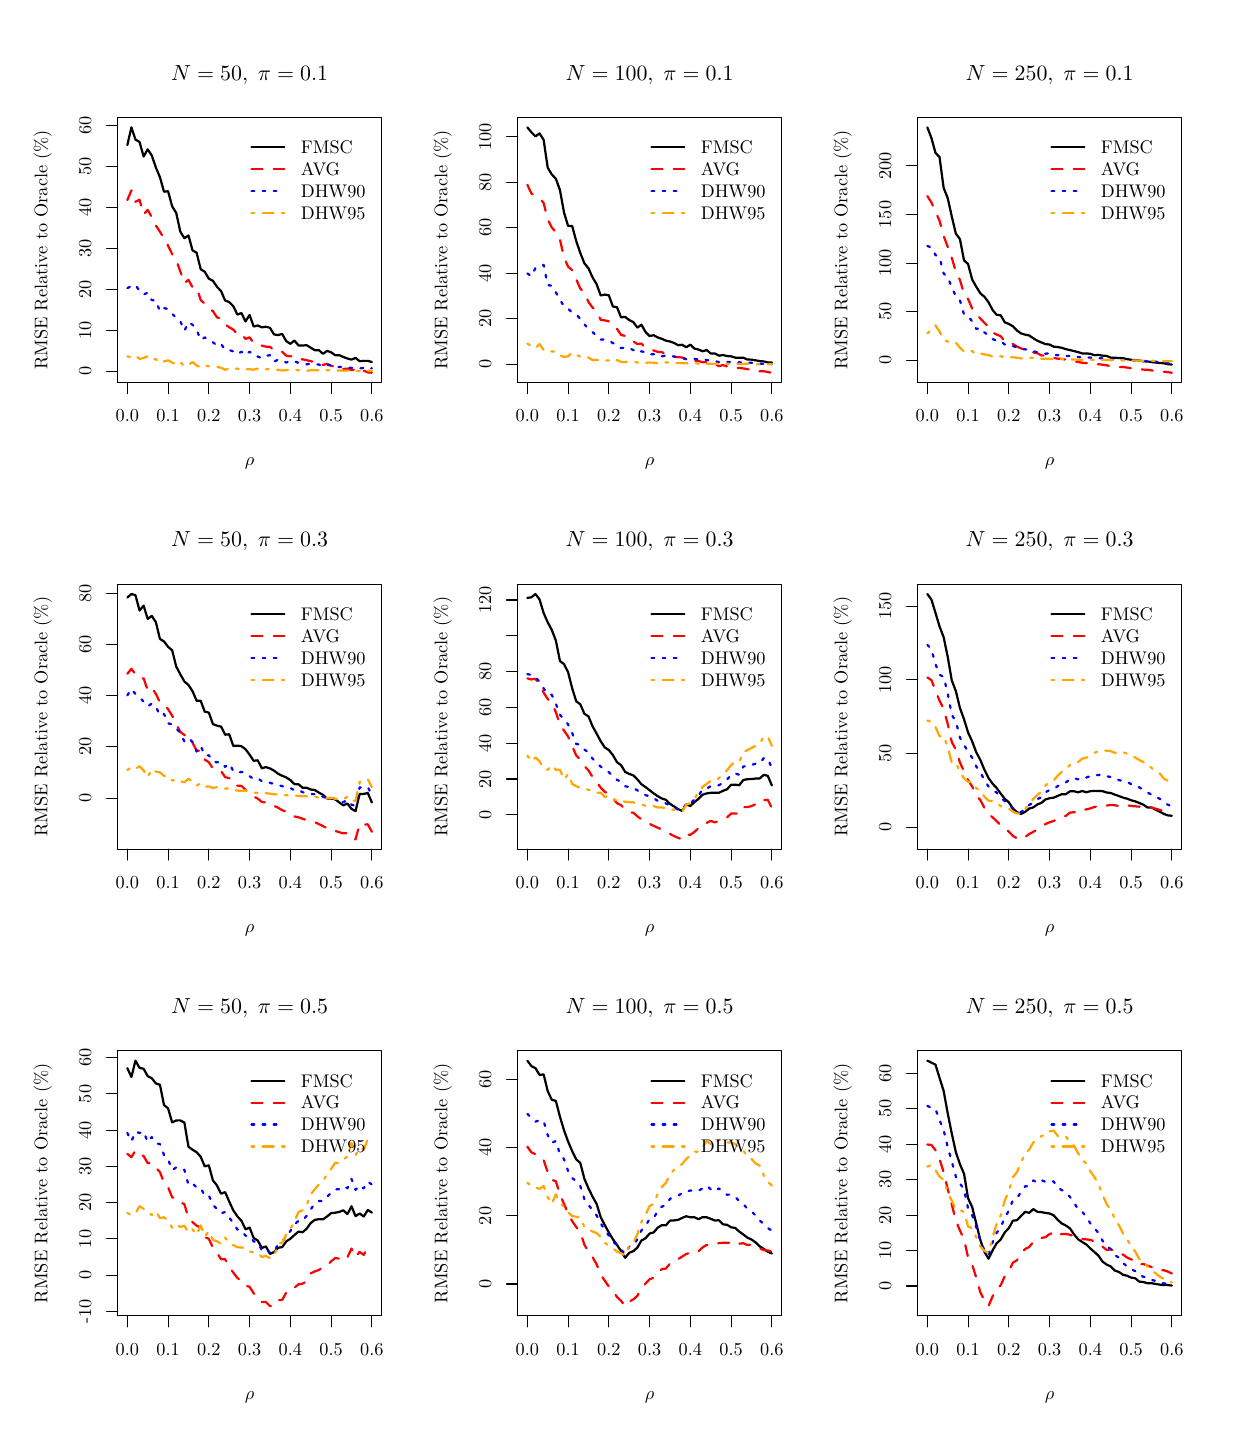
\begin{tikzpicture}[x=1pt,y=1pt]
\definecolor[named]{fillColor}{rgb}{1.00,1.00,1.00}
\path[use as bounding box,fill=fillColor,fill opacity=0.00] (0,0) rectangle (433.62,505.89);
\begin{scope}
\path[clip] ( 32.47,377.65) rectangle (127.91,473.42);
\definecolor[named]{drawColor}{rgb}{0.00,0.00,0.00}

\path[draw=drawColor,line width= 0.8pt,line join=round,line cap=round] ( 36.01,463.45) --
	( 37.48,469.87) --
	( 38.95,465.44) --
	( 40.42,464.59) --
	( 41.90,459.31) --
	( 43.37,461.93) --
	( 44.84,459.70) --
	( 46.32,455.37) --
	( 47.79,451.87) --
	( 49.26,446.61) --
	( 50.73,446.79) --
	( 52.21,441.33) --
	( 53.68,438.94) --
	( 55.15,432.18) --
	( 56.63,429.82) --
	( 58.10,430.80) --
	( 59.57,425.42) --
	( 61.04,424.57) --
	( 62.52,418.60) --
	( 63.99,417.69) --
	( 65.46,415.19) --
	( 66.93,414.43) --
	( 68.41,412.24) --
	( 69.88,410.70) --
	( 71.35,407.29) --
	( 72.83,406.72) --
	( 74.30,405.27) --
	( 75.77,402.21) --
	( 77.24,402.77) --
	( 78.72,399.74) --
	( 80.19,402.08) --
	( 81.66,397.90) --
	( 83.14,398.26) --
	( 84.61,397.60) --
	( 86.08,397.82) --
	( 87.55,397.44) --
	( 89.03,395.02) --
	( 90.50,394.81) --
	( 91.97,395.21) --
	( 93.44,392.60) --
	( 94.92,391.63) --
	( 96.39,392.83) --
	( 97.86,391.07) --
	( 99.34,391.03) --
	(100.81,391.15) --
	(102.28,390.24) --
	(103.75,389.35) --
	(105.23,389.36) --
	(106.70,388.02) --
	(108.17,389.10) --
	(109.65,388.57) --
	(111.12,387.54) --
	(112.59,387.54) --
	(114.06,386.89) --
	(115.54,386.34) --
	(117.01,385.94) --
	(118.48,386.56) --
	(119.95,385.36) --
	(121.43,385.49) --
	(122.90,385.48) --
	(124.37,385.08);
\end{scope}
\begin{scope}
\path[clip] (  0.00,  0.00) rectangle (433.62,505.89);
\definecolor[named]{drawColor}{rgb}{0.00,0.00,0.00}

\path[draw=drawColor,line width= 0.4pt,line join=round,line cap=round] ( 36.01,377.65) -- (124.37,377.65);

\path[draw=drawColor,line width= 0.4pt,line join=round,line cap=round] ( 36.01,377.65) -- ( 36.01,373.69);

\path[draw=drawColor,line width= 0.4pt,line join=round,line cap=round] ( 50.73,377.65) -- ( 50.73,373.69);

\path[draw=drawColor,line width= 0.4pt,line join=round,line cap=round] ( 65.46,377.65) -- ( 65.46,373.69);

\path[draw=drawColor,line width= 0.4pt,line join=round,line cap=round] ( 80.19,377.65) -- ( 80.19,373.69);

\path[draw=drawColor,line width= 0.4pt,line join=round,line cap=round] ( 94.92,377.65) -- ( 94.92,373.69);

\path[draw=drawColor,line width= 0.4pt,line join=round,line cap=round] (109.65,377.65) -- (109.65,373.69);

\path[draw=drawColor,line width= 0.4pt,line join=round,line cap=round] (124.37,377.65) -- (124.37,373.69);

\node[text=drawColor,anchor=base,inner sep=0pt, outer sep=0pt, scale=  0.66] at ( 36.01,363.40) {0.0};

\node[text=drawColor,anchor=base,inner sep=0pt, outer sep=0pt, scale=  0.66] at ( 50.73,363.40) {0.1};

\node[text=drawColor,anchor=base,inner sep=0pt, outer sep=0pt, scale=  0.66] at ( 65.46,363.40) {0.2};

\node[text=drawColor,anchor=base,inner sep=0pt, outer sep=0pt, scale=  0.66] at ( 80.19,363.40) {0.3};

\node[text=drawColor,anchor=base,inner sep=0pt, outer sep=0pt, scale=  0.66] at ( 94.92,363.40) {0.4};

\node[text=drawColor,anchor=base,inner sep=0pt, outer sep=0pt, scale=  0.66] at (109.65,363.40) {0.5};

\node[text=drawColor,anchor=base,inner sep=0pt, outer sep=0pt, scale=  0.66] at (124.37,363.40) {0.6};

\path[draw=drawColor,line width= 0.4pt,line join=round,line cap=round] ( 32.47,381.77) -- ( 32.47,470.63);

\path[draw=drawColor,line width= 0.4pt,line join=round,line cap=round] ( 32.47,381.77) -- ( 28.51,381.77);

\path[draw=drawColor,line width= 0.4pt,line join=round,line cap=round] ( 32.47,396.58) -- ( 28.51,396.58);

\path[draw=drawColor,line width= 0.4pt,line join=round,line cap=round] ( 32.47,411.39) -- ( 28.51,411.39);

\path[draw=drawColor,line width= 0.4pt,line join=round,line cap=round] ( 32.47,426.20) -- ( 28.51,426.20);

\path[draw=drawColor,line width= 0.4pt,line join=round,line cap=round] ( 32.47,441.01) -- ( 28.51,441.01);

\path[draw=drawColor,line width= 0.4pt,line join=round,line cap=round] ( 32.47,455.82) -- ( 28.51,455.82);

\path[draw=drawColor,line width= 0.4pt,line join=round,line cap=round] ( 32.47,470.63) -- ( 28.51,470.63);

\node[text=drawColor,rotate= 90.00,anchor=base,inner sep=0pt, outer sep=0pt, scale=  0.66] at ( 22.97,381.77) {0};

\node[text=drawColor,rotate= 90.00,anchor=base,inner sep=0pt, outer sep=0pt, scale=  0.66] at ( 22.97,396.58) {10};

\node[text=drawColor,rotate= 90.00,anchor=base,inner sep=0pt, outer sep=0pt, scale=  0.66] at ( 22.97,411.39) {20};

\node[text=drawColor,rotate= 90.00,anchor=base,inner sep=0pt, outer sep=0pt, scale=  0.66] at ( 22.97,426.20) {30};

\node[text=drawColor,rotate= 90.00,anchor=base,inner sep=0pt, outer sep=0pt, scale=  0.66] at ( 22.97,441.01) {40};

\node[text=drawColor,rotate= 90.00,anchor=base,inner sep=0pt, outer sep=0pt, scale=  0.66] at ( 22.97,455.82) {50};

\node[text=drawColor,rotate= 90.00,anchor=base,inner sep=0pt, outer sep=0pt, scale=  0.66] at ( 22.97,470.63) {60};

\path[draw=drawColor,line width= 0.4pt,line join=round,line cap=round] ( 32.47,377.65) --
	(127.91,377.65) --
	(127.91,473.42) --
	( 32.47,473.42) --
	( 32.47,377.65);
\end{scope}
\begin{scope}
\path[clip] (  0.00,337.26) rectangle (144.54,505.89);
\definecolor[named]{drawColor}{rgb}{0.00,0.00,0.00}

\node[text=drawColor,anchor=base,inner sep=0pt, outer sep=0pt, scale=  0.79] at ( 80.19,486.92) {\bfseries $N=50, \;\pi=0.1$};

\node[text=drawColor,anchor=base,inner sep=0pt, outer sep=0pt, scale=  0.66] at ( 80.19,347.56) {$\rho$};

\node[text=drawColor,rotate= 90.00,anchor=base,inner sep=0pt, outer sep=0pt, scale=  0.66] at (  7.13,425.53) {RMSE Relative to Oracle (\%)};
\end{scope}
\begin{scope}
\path[clip] ( 32.47,377.65) rectangle (127.91,473.42);
\definecolor[named]{drawColor}{rgb}{1.00,0.00,0.00}

\path[draw=drawColor,line width= 0.8pt,dash pattern=on 4pt off 4pt ,line join=round,line cap=round] ( 36.01,443.58) --
	( 37.48,447.07) --
	( 38.95,442.97) --
	( 40.42,443.72) --
	( 41.90,438.41) --
	( 43.37,440.05) --
	( 44.84,437.45) --
	( 46.32,434.36) --
	( 47.79,432.15) --
	( 49.26,429.75) --
	( 50.73,427.09) --
	( 52.21,424.06) --
	( 53.68,421.90) --
	( 55.15,417.80) --
	( 56.63,413.55) --
	( 58.10,414.77) --
	( 59.57,412.02) --
	( 61.04,411.92) --
	( 62.52,407.47) --
	( 63.99,406.10) --
	( 65.46,404.39) --
	( 66.93,403.48) --
	( 68.41,401.20) --
	( 69.88,400.83) --
	( 71.35,398.67) --
	( 72.83,397.63) --
	( 74.30,396.79) --
	( 75.77,395.14) --
	( 77.24,395.27) --
	( 78.72,393.41) --
	( 80.19,393.98) --
	( 81.66,391.95) --
	( 83.14,391.64) --
	( 84.61,391.01) --
	( 86.08,390.62) --
	( 87.55,390.60) --
	( 89.03,389.23) --
	( 90.50,388.66) --
	( 91.97,388.75) --
	( 93.44,387.36) --
	( 94.92,387.10) --
	( 96.39,387.22) --
	( 97.86,386.28) --
	( 99.34,386.04) --
	(100.81,385.71) --
	(102.28,385.38) --
	(103.75,384.93) --
	(105.23,384.98) --
	(106.70,384.00) --
	(108.17,384.43) --
	(109.65,383.68) --
	(111.12,383.54) --
	(112.59,383.54) --
	(114.06,382.56) --
	(115.54,382.70) --
	(117.01,382.12) --
	(118.48,382.48) --
	(119.95,381.49) --
	(121.43,381.97) --
	(122.90,381.31) --
	(124.37,381.20);
\definecolor[named]{drawColor}{rgb}{0.00,0.00,1.00}

\path[draw=drawColor,line width= 0.8pt,dash pattern=on 1pt off 3pt ,line join=round,line cap=round] ( 36.01,411.78) --
	( 37.48,412.47) --
	( 38.95,412.89) --
	( 40.42,410.77) --
	( 41.90,409.47) --
	( 43.37,410.11) --
	( 44.84,407.44) --
	( 46.32,407.29) --
	( 47.79,403.35) --
	( 49.26,404.56) --
	( 50.73,404.21) --
	( 52.21,402.49) --
	( 53.68,401.01) --
	( 55.15,399.82) --
	( 56.63,396.34) --
	( 58.10,399.40) --
	( 59.57,398.53) --
	( 61.04,396.75) --
	( 62.52,393.03) --
	( 63.99,393.94) --
	( 65.46,393.25) --
	( 66.93,392.19) --
	( 68.41,391.07) --
	( 69.88,391.62) --
	( 71.35,389.45) --
	( 72.83,389.41) --
	( 74.30,388.88) --
	( 75.77,387.91) --
	( 77.24,388.80) --
	( 78.72,387.55) --
	( 80.19,388.84) --
	( 81.66,387.36) --
	( 83.14,387.06) --
	( 84.61,386.46) --
	( 86.08,387.34) --
	( 87.55,387.52) --
	( 89.03,385.19) --
	( 90.50,385.95) --
	( 91.97,385.47) --
	( 93.44,384.87) --
	( 94.92,385.46) --
	( 96.39,385.36) --
	( 97.86,384.76) --
	( 99.34,384.69) --
	(100.81,384.27) --
	(102.28,384.39) --
	(103.75,384.32) --
	(105.23,384.15) --
	(106.70,383.48) --
	(108.17,384.04) --
	(109.65,383.90) --
	(111.12,383.31) --
	(112.59,383.30) --
	(114.06,383.34) --
	(115.54,383.06) --
	(117.01,382.95) --
	(118.48,383.01) --
	(119.95,382.74) --
	(121.43,382.94) --
	(122.90,382.48) --
	(124.37,382.82);
\definecolor[named]{drawColor}{rgb}{1.00,0.65,0.00}

\path[draw=drawColor,line width= 0.8pt,dash pattern=on 1pt off 3pt on 4pt off 3pt ,line join=round,line cap=round] ( 36.01,387.13) --
	( 37.48,386.77) --
	( 38.95,387.41) --
	( 40.42,386.19) --
	( 41.90,386.53) --
	( 43.37,387.20) --
	( 44.84,386.00) --
	( 46.32,386.11) --
	( 47.79,384.75) --
	( 49.26,385.27) --
	( 50.73,385.68) --
	( 52.21,384.89) --
	( 53.68,384.20) --
	( 55.15,385.02) --
	( 56.63,383.47) --
	( 58.10,383.99) --
	( 59.57,385.09) --
	( 61.04,383.85) --
	( 62.52,383.13) --
	( 63.99,383.89) --
	( 65.46,383.51) --
	( 66.93,383.53) --
	( 68.41,383.34) --
	( 69.88,382.99) --
	( 71.35,382.26) --
	( 72.83,382.71) --
	( 74.30,382.97) --
	( 75.77,382.59) --
	( 77.24,382.62) --
	( 78.72,382.55) --
	( 80.19,382.45) --
	( 81.66,382.30) --
	( 83.14,382.69) --
	( 84.61,382.48) --
	( 86.08,382.46) --
	( 87.55,382.54) --
	( 89.03,382.24) --
	( 90.50,382.25) --
	( 91.97,382.01) --
	( 93.44,382.12) --
	( 94.92,382.34) --
	( 96.39,382.18) --
	( 97.86,382.11) --
	( 99.34,381.97) --
	(100.81,381.91) --
	(102.28,382.09) --
	(103.75,382.08) --
	(105.23,382.07) --
	(106.70,382.05) --
	(108.17,382.11) --
	(109.65,381.99) --
	(111.12,381.95) --
	(112.59,381.99) --
	(114.06,381.95) --
	(115.54,381.96) --
	(117.01,381.95) --
	(118.48,381.85) --
	(119.95,381.80) --
	(121.43,381.88) --
	(122.90,381.86) --
	(124.37,382.01);
\definecolor[named]{drawColor}{rgb}{0.00,0.00,0.00}

\path[draw=drawColor,line width= 0.8pt,line join=round,line cap=round] ( 80.89,462.63) -- ( 92.77,462.63);
\definecolor[named]{drawColor}{rgb}{1.00,0.00,0.00}

\path[draw=drawColor,line width= 0.8pt,dash pattern=on 4pt off 4pt ,line join=round,line cap=round] ( 80.89,454.71) -- ( 92.77,454.71);
\definecolor[named]{drawColor}{rgb}{0.00,0.00,1.00}

\path[draw=drawColor,line width= 0.8pt,dash pattern=on 1pt off 3pt ,line join=round,line cap=round] ( 80.89,446.79) -- ( 92.77,446.79);
\definecolor[named]{drawColor}{rgb}{1.00,0.65,0.00}

\path[draw=drawColor,line width= 0.8pt,dash pattern=on 1pt off 3pt on 4pt off 3pt ,line join=round,line cap=round] ( 80.89,438.87) -- ( 92.77,438.87);
\definecolor[named]{drawColor}{rgb}{0.00,0.00,0.00}

\node[text=drawColor,anchor=base west,inner sep=0pt, outer sep=0pt, scale=  0.66] at ( 98.71,460.35) {FMSC};

\node[text=drawColor,anchor=base west,inner sep=0pt, outer sep=0pt, scale=  0.66] at ( 98.71,452.43) {AVG};

\node[text=drawColor,anchor=base west,inner sep=0pt, outer sep=0pt, scale=  0.66] at ( 98.71,444.51) {DHW90};

\node[text=drawColor,anchor=base west,inner sep=0pt, outer sep=0pt, scale=  0.66] at ( 98.71,436.59) {DHW95};
\end{scope}
\begin{scope}
\path[clip] ( 32.47,209.02) rectangle (127.91,304.79);
\definecolor[named]{drawColor}{rgb}{0.00,0.00,0.00}

\path[draw=drawColor,line width= 0.8pt,line join=round,line cap=round] ( 36.01,299.95) --
	( 37.48,301.24) --
	( 38.95,300.84) --
	( 40.42,295.28) --
	( 41.90,297.03) --
	( 43.37,292.22) --
	( 44.84,293.34) --
	( 46.32,291.08) --
	( 47.79,285.01) --
	( 49.26,284.10) --
	( 50.73,282.17) --
	( 52.21,280.90) --
	( 53.68,275.03) --
	( 55.15,272.25) --
	( 56.63,269.62) --
	( 58.10,268.37) --
	( 59.57,266.12) --
	( 61.04,262.68) --
	( 62.52,262.66) --
	( 63.99,258.72) --
	( 65.46,258.40) --
	( 66.93,254.25) --
	( 68.41,253.67) --
	( 69.88,253.33) --
	( 71.35,250.39) --
	( 72.83,250.57) --
	( 74.30,246.34) --
	( 75.77,246.46) --
	( 77.24,246.24) --
	( 78.72,245.15) --
	( 80.19,243.18) --
	( 81.66,240.96) --
	( 83.14,241.16) --
	( 84.61,238.25) --
	( 86.08,238.70) --
	( 87.55,238.22) --
	( 89.03,237.40) --
	( 90.50,236.27) --
	( 91.97,235.57) --
	( 93.44,234.95) --
	( 94.92,234.00) --
	( 96.39,232.55) --
	( 97.86,232.49) --
	( 99.34,231.26) --
	(100.81,231.23) --
	(102.28,230.59) --
	(103.75,230.42) --
	(105.23,229.46) --
	(106.70,228.69) --
	(108.17,227.34) --
	(109.65,227.35) --
	(111.12,227.05) --
	(112.59,225.91) --
	(114.06,224.88) --
	(115.54,225.54) --
	(117.01,223.59) --
	(118.48,222.79) --
	(119.95,229.01) --
	(121.43,229.00) --
	(122.90,229.35) --
	(124.37,225.93);
\end{scope}
\begin{scope}
\path[clip] (  0.00,  0.00) rectangle (433.62,505.89);
\definecolor[named]{drawColor}{rgb}{0.00,0.00,0.00}

\path[draw=drawColor,line width= 0.4pt,line join=round,line cap=round] ( 36.01,209.02) -- (124.37,209.02);

\path[draw=drawColor,line width= 0.4pt,line join=round,line cap=round] ( 36.01,209.02) -- ( 36.01,205.06);

\path[draw=drawColor,line width= 0.4pt,line join=round,line cap=round] ( 50.73,209.02) -- ( 50.73,205.06);

\path[draw=drawColor,line width= 0.4pt,line join=round,line cap=round] ( 65.46,209.02) -- ( 65.46,205.06);

\path[draw=drawColor,line width= 0.4pt,line join=round,line cap=round] ( 80.19,209.02) -- ( 80.19,205.06);

\path[draw=drawColor,line width= 0.4pt,line join=round,line cap=round] ( 94.92,209.02) -- ( 94.92,205.06);

\path[draw=drawColor,line width= 0.4pt,line join=round,line cap=round] (109.65,209.02) -- (109.65,205.06);

\path[draw=drawColor,line width= 0.4pt,line join=round,line cap=round] (124.37,209.02) -- (124.37,205.06);

\node[text=drawColor,anchor=base,inner sep=0pt, outer sep=0pt, scale=  0.66] at ( 36.01,194.77) {0.0};

\node[text=drawColor,anchor=base,inner sep=0pt, outer sep=0pt, scale=  0.66] at ( 50.73,194.77) {0.1};

\node[text=drawColor,anchor=base,inner sep=0pt, outer sep=0pt, scale=  0.66] at ( 65.46,194.77) {0.2};

\node[text=drawColor,anchor=base,inner sep=0pt, outer sep=0pt, scale=  0.66] at ( 80.19,194.77) {0.3};

\node[text=drawColor,anchor=base,inner sep=0pt, outer sep=0pt, scale=  0.66] at ( 94.92,194.77) {0.4};

\node[text=drawColor,anchor=base,inner sep=0pt, outer sep=0pt, scale=  0.66] at (109.65,194.77) {0.5};

\node[text=drawColor,anchor=base,inner sep=0pt, outer sep=0pt, scale=  0.66] at (124.37,194.77) {0.6};

\path[draw=drawColor,line width= 0.4pt,line join=round,line cap=round] ( 32.47,227.50) -- ( 32.47,301.57);

\path[draw=drawColor,line width= 0.4pt,line join=round,line cap=round] ( 32.47,227.50) -- ( 28.51,227.50);

\path[draw=drawColor,line width= 0.4pt,line join=round,line cap=round] ( 32.47,246.02) -- ( 28.51,246.02);

\path[draw=drawColor,line width= 0.4pt,line join=round,line cap=round] ( 32.47,264.54) -- ( 28.51,264.54);

\path[draw=drawColor,line width= 0.4pt,line join=round,line cap=round] ( 32.47,283.05) -- ( 28.51,283.05);

\path[draw=drawColor,line width= 0.4pt,line join=round,line cap=round] ( 32.47,301.57) -- ( 28.51,301.57);

\node[text=drawColor,rotate= 90.00,anchor=base,inner sep=0pt, outer sep=0pt, scale=  0.66] at ( 22.97,227.50) {0};

\node[text=drawColor,rotate= 90.00,anchor=base,inner sep=0pt, outer sep=0pt, scale=  0.66] at ( 22.97,246.02) {20};

\node[text=drawColor,rotate= 90.00,anchor=base,inner sep=0pt, outer sep=0pt, scale=  0.66] at ( 22.97,264.54) {40};

\node[text=drawColor,rotate= 90.00,anchor=base,inner sep=0pt, outer sep=0pt, scale=  0.66] at ( 22.97,283.05) {60};

\node[text=drawColor,rotate= 90.00,anchor=base,inner sep=0pt, outer sep=0pt, scale=  0.66] at ( 22.97,301.57) {80};

\path[draw=drawColor,line width= 0.4pt,line join=round,line cap=round] ( 32.47,209.02) --
	(127.91,209.02) --
	(127.91,304.79) --
	( 32.47,304.79) --
	( 32.47,209.02);
\end{scope}
\begin{scope}
\path[clip] (  0.00,168.63) rectangle (144.54,337.26);
\definecolor[named]{drawColor}{rgb}{0.00,0.00,0.00}

\node[text=drawColor,anchor=base,inner sep=0pt, outer sep=0pt, scale=  0.79] at ( 80.19,318.29) {\bfseries $N=50, \;\pi=0.3$};

\node[text=drawColor,anchor=base,inner sep=0pt, outer sep=0pt, scale=  0.66] at ( 80.19,178.93) {$\rho$};

\node[text=drawColor,rotate= 90.00,anchor=base,inner sep=0pt, outer sep=0pt, scale=  0.66] at (  7.13,256.90) {RMSE Relative to Oracle (\%)};
\end{scope}
\begin{scope}
\path[clip] ( 32.47,209.02) rectangle (127.91,304.79);
\definecolor[named]{drawColor}{rgb}{1.00,0.00,0.00}

\path[draw=drawColor,line width= 0.8pt,dash pattern=on 4pt off 4pt ,line join=round,line cap=round] ( 36.01,272.41) --
	( 37.48,274.20) --
	( 38.95,272.26) --
	( 40.42,270.71) --
	( 41.90,270.76) --
	( 43.37,266.47) --
	( 44.84,267.38) --
	( 46.32,265.14) --
	( 47.79,262.13) --
	( 49.26,261.41) --
	( 50.73,259.65) --
	( 52.21,257.26) --
	( 53.68,254.26) --
	( 55.15,251.41) --
	( 56.63,250.32) --
	( 58.10,249.56) --
	( 59.57,247.51) --
	( 61.04,244.71) --
	( 62.52,244.54) --
	( 63.99,241.42) --
	( 65.46,240.49) --
	( 66.93,238.15) --
	( 68.41,237.62) --
	( 69.88,237.25) --
	( 71.35,235.07) --
	( 72.83,234.70) --
	( 74.30,232.46) --
	( 75.77,232.01) --
	( 77.24,231.91) --
	( 78.72,230.49) --
	( 80.19,229.04) --
	( 81.66,228.06) --
	( 83.14,227.30) --
	( 84.61,226.10) --
	( 86.08,225.88) --
	( 87.55,225.55) --
	( 89.03,224.70) --
	( 90.50,224.02) --
	( 91.97,223.12) --
	( 93.44,222.61) --
	( 94.92,222.04) --
	( 96.39,220.88) --
	( 97.86,220.54) --
	( 99.34,220.04) --
	(100.81,219.52) --
	(102.28,219.12) --
	(103.75,218.82) --
	(105.23,218.11) --
	(106.70,217.39) --
	(108.17,216.59) --
	(109.65,216.51) --
	(111.12,215.63) --
	(112.59,215.17) --
	(114.06,214.74) --
	(115.54,214.87) --
	(117.01,213.04) --
	(118.48,212.57) --
	(119.95,218.08) --
	(121.43,217.93) --
	(122.90,218.02) --
	(124.37,215.31);
\definecolor[named]{drawColor}{rgb}{0.00,0.00,1.00}

\path[draw=drawColor,line width= 0.8pt,dash pattern=on 1pt off 3pt ,line join=round,line cap=round] ( 36.01,264.62) --
	( 37.48,266.93) --
	( 38.95,265.10) --
	( 40.42,263.96) --
	( 41.90,262.32) --
	( 43.37,260.62) --
	( 44.84,261.65) --
	( 46.32,260.57) --
	( 47.79,257.35) --
	( 49.26,257.92) --
	( 50.73,254.51) --
	( 52.21,254.13) --
	( 53.68,252.71) --
	( 55.15,251.00) --
	( 56.63,248.00) --
	( 58.10,249.19) --
	( 59.57,247.74) --
	( 61.04,244.32) --
	( 62.52,246.35) --
	( 63.99,242.92) --
	( 65.46,242.94) --
	( 66.93,240.75) --
	( 68.41,240.41) --
	( 69.88,240.64) --
	( 71.35,238.78) --
	( 72.83,240.00) --
	( 74.30,237.30) --
	( 75.77,236.60) --
	( 77.24,236.99) --
	( 78.72,236.48) --
	( 80.19,235.41) --
	( 81.66,234.38) --
	( 83.14,234.68) --
	( 84.61,233.56) --
	( 86.08,233.26) --
	( 87.55,233.03) --
	( 89.03,232.56) --
	( 90.50,232.25) --
	( 91.97,231.81) --
	( 93.44,231.20) --
	( 94.92,231.12) --
	( 96.39,230.38) --
	( 97.86,230.52) --
	( 99.34,229.59) --
	(100.81,229.44) --
	(102.28,228.97) --
	(103.75,228.90) --
	(105.23,228.22) --
	(106.70,228.00) --
	(108.17,227.28) --
	(109.65,227.82) --
	(111.12,227.07) --
	(112.59,226.47) --
	(114.06,226.01) --
	(115.54,226.84) --
	(117.01,225.12) --
	(118.48,224.67) --
	(119.95,231.34) --
	(121.43,231.28) --
	(122.90,231.46) --
	(124.37,228.62);
\definecolor[named]{drawColor}{rgb}{1.00,0.65,0.00}

\path[draw=drawColor,line width= 0.8pt,dash pattern=on 1pt off 3pt on 4pt off 3pt ,line join=round,line cap=round] ( 36.01,237.65) --
	( 37.48,238.64) --
	( 38.95,238.03) --
	( 40.42,239.01) --
	( 41.90,237.49) --
	( 43.37,234.97) --
	( 44.84,237.97) --
	( 46.32,237.10) --
	( 47.79,236.75) --
	( 49.26,235.52) --
	( 50.73,235.41) --
	( 52.21,233.79) --
	( 53.68,234.33) --
	( 55.15,233.56) --
	( 56.63,233.20) --
	( 58.10,234.49) --
	( 59.57,233.37) --
	( 61.04,232.03) --
	( 62.52,232.78) --
	( 63.99,231.56) --
	( 65.46,231.72) --
	( 66.93,231.14) --
	( 68.41,231.46) --
	( 69.88,231.36) --
	( 71.35,230.91) --
	( 72.83,231.00) --
	( 74.30,230.45) --
	( 75.77,230.23) --
	( 77.24,230.03) --
	( 78.72,230.26) --
	( 80.19,229.85) --
	( 81.66,229.48) --
	( 83.14,229.43) --
	( 84.61,229.02) --
	( 86.08,229.29) --
	( 87.55,229.08) --
	( 89.03,228.86) --
	( 90.50,228.79) --
	( 91.97,228.66) --
	( 93.44,228.51) --
	( 94.92,228.47) --
	( 96.39,228.40) --
	( 97.86,228.28) --
	( 99.34,228.14) --
	(100.81,228.12) --
	(102.28,228.11) --
	(103.75,227.95) --
	(105.23,227.64) --
	(106.70,227.54) --
	(108.17,227.42) --
	(109.65,227.64) --
	(111.12,227.24) --
	(112.59,227.04) --
	(114.06,226.91) --
	(115.54,228.06) --
	(117.01,226.62) --
	(118.48,226.47) --
	(119.95,233.36) --
	(121.43,233.76) --
	(122.90,234.35) --
	(124.37,231.42);
\definecolor[named]{drawColor}{rgb}{0.00,0.00,0.00}

\path[draw=drawColor,line width= 0.8pt,line join=round,line cap=round] ( 80.89,294.00) -- ( 92.77,294.00);
\definecolor[named]{drawColor}{rgb}{1.00,0.00,0.00}

\path[draw=drawColor,line width= 0.8pt,dash pattern=on 4pt off 4pt ,line join=round,line cap=round] ( 80.89,286.08) -- ( 92.77,286.08);
\definecolor[named]{drawColor}{rgb}{0.00,0.00,1.00}

\path[draw=drawColor,line width= 0.8pt,dash pattern=on 1pt off 3pt ,line join=round,line cap=round] ( 80.89,278.16) -- ( 92.77,278.16);
\definecolor[named]{drawColor}{rgb}{1.00,0.65,0.00}

\path[draw=drawColor,line width= 0.8pt,dash pattern=on 1pt off 3pt on 4pt off 3pt ,line join=round,line cap=round] ( 80.89,270.24) -- ( 92.77,270.24);
\definecolor[named]{drawColor}{rgb}{0.00,0.00,0.00}

\node[text=drawColor,anchor=base west,inner sep=0pt, outer sep=0pt, scale=  0.66] at ( 98.71,291.72) {FMSC};

\node[text=drawColor,anchor=base west,inner sep=0pt, outer sep=0pt, scale=  0.66] at ( 98.71,283.80) {AVG};

\node[text=drawColor,anchor=base west,inner sep=0pt, outer sep=0pt, scale=  0.66] at ( 98.71,275.88) {DHW90};

\node[text=drawColor,anchor=base west,inner sep=0pt, outer sep=0pt, scale=  0.66] at ( 98.71,267.96) {DHW95};
\end{scope}
\begin{scope}
\path[clip] ( 32.47, 40.39) rectangle (127.91,136.16);
\definecolor[named]{drawColor}{rgb}{0.00,0.00,0.00}

\path[draw=drawColor,line width= 0.8pt,line join=round,line cap=round] ( 36.01,129.91) --
	( 37.48,126.71) --
	( 38.95,132.61) --
	( 40.42,130.02) --
	( 41.90,129.68) --
	( 43.37,127.00) --
	( 44.84,126.29) --
	( 46.32,124.40) --
	( 47.79,123.92) --
	( 49.26,116.57) --
	( 50.73,115.40) --
	( 52.21,110.29) --
	( 53.68,111.03) --
	( 55.15,111.04) --
	( 56.63,110.25) --
	( 58.10,101.52) --
	( 59.57,100.44) --
	( 61.04, 99.54) --
	( 62.52, 97.89) --
	( 63.99, 94.41) --
	( 65.46, 94.81) --
	( 66.93, 89.37) --
	( 68.41, 87.50) --
	( 69.88, 84.55) --
	( 71.35, 85.11) --
	( 72.83, 81.69) --
	( 74.30, 78.53) --
	( 75.77, 76.36) --
	( 77.24, 74.77) --
	( 78.72, 71.67) --
	( 80.19, 72.30) --
	( 81.66, 68.54) --
	( 83.14, 67.63) --
	( 84.61, 64.96) --
	( 86.08, 65.46) --
	( 87.55, 62.80) --
	( 89.03, 63.44) --
	( 90.50, 64.99) --
	( 91.97, 65.26) --
	( 93.44, 67.30) --
	( 94.92, 68.27) --
	( 96.39, 69.63) --
	( 97.86, 70.83) --
	( 99.34, 70.62) --
	(100.81, 71.89) --
	(102.28, 73.95) --
	(103.75, 75.06) --
	(105.23, 75.37) --
	(106.70, 75.26) --
	(108.17, 76.30) --
	(109.65, 77.52) --
	(111.12, 77.67) --
	(112.59, 77.96) --
	(114.06, 78.55) --
	(115.54, 77.17) --
	(117.01, 80.00) --
	(118.48, 76.45) --
	(119.95, 77.40) --
	(121.43, 76.32) --
	(122.90, 78.67) --
	(124.37, 77.72);
\end{scope}
\begin{scope}
\path[clip] (  0.00,  0.00) rectangle (433.62,505.89);
\definecolor[named]{drawColor}{rgb}{0.00,0.00,0.00}

\path[draw=drawColor,line width= 0.4pt,line join=round,line cap=round] ( 36.01, 40.39) -- (124.37, 40.39);

\path[draw=drawColor,line width= 0.4pt,line join=round,line cap=round] ( 36.01, 40.39) -- ( 36.01, 36.43);

\path[draw=drawColor,line width= 0.4pt,line join=round,line cap=round] ( 50.73, 40.39) -- ( 50.73, 36.43);

\path[draw=drawColor,line width= 0.4pt,line join=round,line cap=round] ( 65.46, 40.39) -- ( 65.46, 36.43);

\path[draw=drawColor,line width= 0.4pt,line join=round,line cap=round] ( 80.19, 40.39) -- ( 80.19, 36.43);

\path[draw=drawColor,line width= 0.4pt,line join=round,line cap=round] ( 94.92, 40.39) -- ( 94.92, 36.43);

\path[draw=drawColor,line width= 0.4pt,line join=round,line cap=round] (109.65, 40.39) -- (109.65, 36.43);

\path[draw=drawColor,line width= 0.4pt,line join=round,line cap=round] (124.37, 40.39) -- (124.37, 36.43);

\node[text=drawColor,anchor=base,inner sep=0pt, outer sep=0pt, scale=  0.66] at ( 36.01, 26.14) {0.0};

\node[text=drawColor,anchor=base,inner sep=0pt, outer sep=0pt, scale=  0.66] at ( 50.73, 26.14) {0.1};

\node[text=drawColor,anchor=base,inner sep=0pt, outer sep=0pt, scale=  0.66] at ( 65.46, 26.14) {0.2};

\node[text=drawColor,anchor=base,inner sep=0pt, outer sep=0pt, scale=  0.66] at ( 80.19, 26.14) {0.3};

\node[text=drawColor,anchor=base,inner sep=0pt, outer sep=0pt, scale=  0.66] at ( 94.92, 26.14) {0.4};

\node[text=drawColor,anchor=base,inner sep=0pt, outer sep=0pt, scale=  0.66] at (109.65, 26.14) {0.5};

\node[text=drawColor,anchor=base,inner sep=0pt, outer sep=0pt, scale=  0.66] at (124.37, 26.14) {0.6};

\path[draw=drawColor,line width= 0.4pt,line join=round,line cap=round] ( 32.47, 42.03) -- ( 32.47,133.69);

\path[draw=drawColor,line width= 0.4pt,line join=round,line cap=round] ( 32.47, 42.03) -- ( 28.51, 42.03);

\path[draw=drawColor,line width= 0.4pt,line join=round,line cap=round] ( 32.47, 55.13) -- ( 28.51, 55.13);

\path[draw=drawColor,line width= 0.4pt,line join=round,line cap=round] ( 32.47, 68.22) -- ( 28.51, 68.22);

\path[draw=drawColor,line width= 0.4pt,line join=round,line cap=round] ( 32.47, 81.32) -- ( 28.51, 81.32);

\path[draw=drawColor,line width= 0.4pt,line join=round,line cap=round] ( 32.47, 94.41) -- ( 28.51, 94.41);

\path[draw=drawColor,line width= 0.4pt,line join=round,line cap=round] ( 32.47,107.50) -- ( 28.51,107.50);

\path[draw=drawColor,line width= 0.4pt,line join=round,line cap=round] ( 32.47,120.60) -- ( 28.51,120.60);

\path[draw=drawColor,line width= 0.4pt,line join=round,line cap=round] ( 32.47,133.69) -- ( 28.51,133.69);

\node[text=drawColor,rotate= 90.00,anchor=base,inner sep=0pt, outer sep=0pt, scale=  0.66] at ( 22.97, 42.03) {-10};

\node[text=drawColor,rotate= 90.00,anchor=base,inner sep=0pt, outer sep=0pt, scale=  0.66] at ( 22.97, 55.13) {0};

\node[text=drawColor,rotate= 90.00,anchor=base,inner sep=0pt, outer sep=0pt, scale=  0.66] at ( 22.97, 68.22) {10};

\node[text=drawColor,rotate= 90.00,anchor=base,inner sep=0pt, outer sep=0pt, scale=  0.66] at ( 22.97, 81.32) {20};

\node[text=drawColor,rotate= 90.00,anchor=base,inner sep=0pt, outer sep=0pt, scale=  0.66] at ( 22.97, 94.41) {30};

\node[text=drawColor,rotate= 90.00,anchor=base,inner sep=0pt, outer sep=0pt, scale=  0.66] at ( 22.97,107.50) {40};

\node[text=drawColor,rotate= 90.00,anchor=base,inner sep=0pt, outer sep=0pt, scale=  0.66] at ( 22.97,120.60) {50};

\node[text=drawColor,rotate= 90.00,anchor=base,inner sep=0pt, outer sep=0pt, scale=  0.66] at ( 22.97,133.69) {60};

\path[draw=drawColor,line width= 0.4pt,line join=round,line cap=round] ( 32.47, 40.39) --
	(127.91, 40.39) --
	(127.91,136.16) --
	( 32.47,136.16) --
	( 32.47, 40.39);
\end{scope}
\begin{scope}
\path[clip] (  0.00,  0.00) rectangle (144.54,168.63);
\definecolor[named]{drawColor}{rgb}{0.00,0.00,0.00}

\node[text=drawColor,anchor=base,inner sep=0pt, outer sep=0pt, scale=  0.79] at ( 80.19,149.66) {\bfseries $N=50, \;\pi=0.5$};

\node[text=drawColor,anchor=base,inner sep=0pt, outer sep=0pt, scale=  0.66] at ( 80.19, 10.30) {$\rho$};

\node[text=drawColor,rotate= 90.00,anchor=base,inner sep=0pt, outer sep=0pt, scale=  0.66] at (  7.13, 88.27) {RMSE Relative to Oracle (\%)};
\end{scope}
\begin{scope}
\path[clip] ( 32.47, 40.39) rectangle (127.91,136.16);
\definecolor[named]{drawColor}{rgb}{1.00,0.00,0.00}

\path[draw=drawColor,line width= 0.8pt,dash pattern=on 4pt off 4pt ,line join=round,line cap=round] ( 36.01, 98.94) --
	( 37.48, 97.73) --
	( 38.95,100.16) --
	( 40.42, 98.75) --
	( 41.90, 98.19) --
	( 43.37, 95.59) --
	( 44.84, 95.77) --
	( 46.32, 93.97) --
	( 47.79, 92.36) --
	( 49.26, 88.59) --
	( 50.73, 86.88) --
	( 52.21, 83.22) --
	( 53.68, 83.02) --
	( 55.15, 81.46) --
	( 56.63, 80.76) --
	( 58.10, 75.71) --
	( 59.57, 74.28) --
	( 61.04, 72.99) --
	( 62.52, 72.34) --
	( 63.99, 68.84) --
	( 65.46, 68.24) --
	( 66.93, 65.02) --
	( 68.41, 63.17) --
	( 69.88, 60.88) --
	( 71.35, 60.86) --
	( 72.83, 58.23) --
	( 74.30, 56.04) --
	( 75.77, 54.11) --
	( 77.24, 53.08) --
	( 78.72, 51.30) --
	( 80.19, 50.92) --
	( 81.66, 48.55) --
	( 83.14, 47.33) --
	( 84.61, 45.39) --
	( 86.08, 45.42) --
	( 87.55, 43.94) --
	( 89.03, 44.00) --
	( 90.50, 46.07) --
	( 91.97, 46.15) --
	( 93.44, 48.85) --
	( 94.92, 49.23) --
	( 96.39, 50.58) --
	( 97.86, 51.80) --
	( 99.34, 52.05) --
	(100.81, 52.90) --
	(102.28, 55.75) --
	(103.75, 56.48) --
	(105.23, 56.97) --
	(106.70, 57.97) --
	(108.17, 58.45) --
	(109.65, 60.09) --
	(111.12, 61.31) --
	(112.59, 61.07) --
	(114.06, 62.32) --
	(115.54, 61.55) --
	(117.01, 64.72) --
	(118.48, 61.62) --
	(119.95, 63.51) --
	(121.43, 62.44) --
	(122.90, 65.44) --
	(124.37, 64.58);
\definecolor[named]{drawColor}{rgb}{0.00,0.00,1.00}

\path[draw=drawColor,line width= 0.8pt,dash pattern=on 1pt off 3pt ,line join=round,line cap=round] ( 36.01,106.52) --
	( 37.48,103.48) --
	( 38.95,106.94) --
	( 40.42,106.49) --
	( 41.90,106.94) --
	( 43.37,103.19) --
	( 44.84,105.01) --
	( 46.32,102.77) --
	( 47.79,102.47) --
	( 49.26, 98.54) --
	( 50.73, 96.99) --
	( 52.21, 93.05) --
	( 53.68, 94.05) --
	( 55.15, 93.81) --
	( 56.63, 93.14) --
	( 58.10, 87.75) --
	( 59.57, 88.29) --
	( 61.04, 86.81) --
	( 62.52, 86.65) --
	( 63.99, 83.80) --
	( 65.46, 83.92) --
	( 66.93, 80.49) --
	( 68.41, 79.04) --
	( 69.88, 77.48) --
	( 71.35, 77.92) --
	( 72.83, 75.95) --
	( 74.30, 73.90) --
	( 75.77, 71.63) --
	( 77.24, 71.31) --
	( 78.72, 69.36) --
	( 80.19, 69.21) --
	( 81.66, 67.30) --
	( 83.14, 66.92) --
	( 84.61, 64.09) --
	( 86.08, 64.75) --
	( 87.55, 63.28) --
	( 89.03, 63.36) --
	( 90.50, 66.44) --
	( 91.97, 67.20) --
	( 93.44, 69.16) --
	( 94.92, 71.06) --
	( 96.39, 73.43) --
	( 97.86, 74.74) --
	( 99.34, 74.78) --
	(100.81, 76.57) --
	(102.28, 78.90) --
	(103.75, 80.94) --
	(105.23, 81.90) --
	(106.70, 81.91) --
	(108.17, 83.48) --
	(109.65, 84.81) --
	(111.12, 86.07) --
	(112.59, 86.19) --
	(114.06, 87.18) --
	(115.54, 86.52) --
	(117.01, 89.89) --
	(118.48, 85.93) --
	(119.95, 87.61) --
	(121.43, 86.50) --
	(122.90, 88.96) --
	(124.37, 87.83);
\definecolor[named]{drawColor}{rgb}{1.00,0.65,0.00}

\path[draw=drawColor,line width= 0.8pt,dash pattern=on 1pt off 3pt on 4pt off 3pt ,line join=round,line cap=round] ( 36.01, 77.60) --
	( 37.48, 76.84) --
	( 38.95, 77.47) --
	( 40.42, 80.00) --
	( 41.90, 79.09) --
	( 43.37, 78.20) --
	( 44.84, 76.82) --
	( 46.32, 78.24) --
	( 47.79, 75.73) --
	( 49.26, 76.04) --
	( 50.73, 74.69) --
	( 52.21, 72.25) --
	( 53.68, 73.52) --
	( 55.15, 72.48) --
	( 56.63, 73.00) --
	( 58.10, 70.47) --
	( 59.57, 71.68) --
	( 61.04, 69.72) --
	( 62.52, 73.09) --
	( 63.99, 69.16) --
	( 65.46, 70.90) --
	( 66.93, 67.86) --
	( 68.41, 67.34) --
	( 69.88, 66.47) --
	( 71.35, 68.70) --
	( 72.83, 66.61) --
	( 74.30, 65.91) --
	( 75.77, 65.21) --
	( 77.24, 65.08) --
	( 78.72, 64.98) --
	( 80.19, 63.66) --
	( 81.66, 63.32) --
	( 83.14, 63.17) --
	( 84.61, 61.65) --
	( 86.08, 62.04) --
	( 87.55, 61.27) --
	( 89.03, 61.95) --
	( 90.50, 66.19) --
	( 91.97, 66.97) --
	( 93.44, 69.73) --
	( 94.92, 71.76) --
	( 96.39, 74.50) --
	( 97.86, 77.91) --
	( 99.34, 78.58) --
	(100.81, 80.46) --
	(102.28, 84.27) --
	(103.75, 86.15) --
	(105.23, 87.91) --
	(106.70, 89.02) --
	(108.17, 91.57) --
	(109.65, 93.50) --
	(111.12, 95.70) --
	(112.59, 95.62) --
	(114.06, 96.92) --
	(115.54, 97.94) --
	(117.01,102.92) --
	(118.48, 98.57) --
	(119.95,101.10) --
	(121.43,100.46) --
	(122.90,104.19) --
	(124.37,103.52);
\definecolor[named]{drawColor}{rgb}{0.00,0.00,0.00}

\path[draw=drawColor,line width= 0.8pt,line join=round,line cap=round] ( 80.89,125.37) -- ( 92.77,125.37);
\definecolor[named]{drawColor}{rgb}{1.00,0.00,0.00}

\path[draw=drawColor,line width= 0.8pt,dash pattern=on 4pt off 4pt ,line join=round,line cap=round] ( 80.89,117.45) -- ( 92.77,117.45);
\definecolor[named]{drawColor}{rgb}{0.00,0.00,1.00}

\path[draw=drawColor,line width= 0.8pt,dash pattern=on 1pt off 3pt ,line join=round,line cap=round] ( 80.89,109.53) -- ( 92.77,109.53);
\definecolor[named]{drawColor}{rgb}{1.00,0.65,0.00}

\path[draw=drawColor,line width= 0.8pt,dash pattern=on 1pt off 3pt on 4pt off 3pt ,line join=round,line cap=round] ( 80.89,101.61) -- ( 92.77,101.61);
\definecolor[named]{drawColor}{rgb}{0.00,0.00,0.00}

\node[text=drawColor,anchor=base west,inner sep=0pt, outer sep=0pt, scale=  0.66] at ( 98.71,123.09) {FMSC};

\node[text=drawColor,anchor=base west,inner sep=0pt, outer sep=0pt, scale=  0.66] at ( 98.71,115.17) {AVG};

\node[text=drawColor,anchor=base west,inner sep=0pt, outer sep=0pt, scale=  0.66] at ( 98.71,107.25) {DHW90};

\node[text=drawColor,anchor=base west,inner sep=0pt, outer sep=0pt, scale=  0.66] at ( 98.71, 99.33) {DHW95};
\end{scope}
\begin{scope}
\path[clip] (177.01,377.65) rectangle (272.45,473.42);
\definecolor[named]{drawColor}{rgb}{0.00,0.00,0.00}

\path[draw=drawColor,line width= 0.8pt,line join=round,line cap=round] (180.55,469.87) --
	(182.02,468.08) --
	(183.49,466.61) --
	(184.96,467.68) --
	(186.44,465.36) --
	(187.91,455.31) --
	(189.38,452.86) --
	(190.86,451.27) --
	(192.33,447.24) --
	(193.80,439.11) --
	(195.27,434.26) --
	(196.75,434.21) --
	(198.22,428.76) --
	(199.69,424.47) --
	(201.17,420.74) --
	(202.64,418.93) --
	(204.11,415.67) --
	(205.58,413.20) --
	(207.06,409.11) --
	(208.53,409.44) --
	(210.00,409.16) --
	(211.47,405.13) --
	(212.95,404.87) --
	(214.42,401.21) --
	(215.89,401.38) --
	(217.37,400.23) --
	(218.84,399.52) --
	(220.31,397.50) --
	(221.78,398.55) --
	(223.26,395.91) --
	(224.73,394.45) --
	(226.20,394.77) --
	(227.68,393.93) --
	(229.15,393.46) --
	(230.62,392.80) --
	(232.09,392.49) --
	(233.57,391.97) --
	(235.04,391.13) --
	(236.51,391.30) --
	(237.98,390.40) --
	(239.46,391.35) --
	(240.93,389.92) --
	(242.40,389.57) --
	(243.88,388.95) --
	(245.35,389.41) --
	(246.82,388.14) --
	(248.29,388.18) --
	(249.77,387.35) --
	(251.24,387.60) --
	(252.71,387.22) --
	(254.19,387.13) --
	(255.66,386.65) --
	(257.13,386.63) --
	(258.60,386.62) --
	(260.08,385.96) --
	(261.55,385.93) --
	(263.02,385.68) --
	(264.50,385.41) --
	(265.97,385.29) --
	(267.44,384.93) --
	(268.91,384.91);
\end{scope}
\begin{scope}
\path[clip] (  0.00,  0.00) rectangle (433.62,505.89);
\definecolor[named]{drawColor}{rgb}{0.00,0.00,0.00}

\path[draw=drawColor,line width= 0.4pt,line join=round,line cap=round] (180.55,377.65) -- (268.91,377.65);

\path[draw=drawColor,line width= 0.4pt,line join=round,line cap=round] (180.55,377.65) -- (180.55,373.69);

\path[draw=drawColor,line width= 0.4pt,line join=round,line cap=round] (195.27,377.65) -- (195.27,373.69);

\path[draw=drawColor,line width= 0.4pt,line join=round,line cap=round] (210.00,377.65) -- (210.00,373.69);

\path[draw=drawColor,line width= 0.4pt,line join=round,line cap=round] (224.73,377.65) -- (224.73,373.69);

\path[draw=drawColor,line width= 0.4pt,line join=round,line cap=round] (239.46,377.65) -- (239.46,373.69);

\path[draw=drawColor,line width= 0.4pt,line join=round,line cap=round] (254.19,377.65) -- (254.19,373.69);

\path[draw=drawColor,line width= 0.4pt,line join=round,line cap=round] (268.91,377.65) -- (268.91,373.69);

\node[text=drawColor,anchor=base,inner sep=0pt, outer sep=0pt, scale=  0.66] at (180.55,363.40) {0.0};

\node[text=drawColor,anchor=base,inner sep=0pt, outer sep=0pt, scale=  0.66] at (195.27,363.40) {0.1};

\node[text=drawColor,anchor=base,inner sep=0pt, outer sep=0pt, scale=  0.66] at (210.00,363.40) {0.2};

\node[text=drawColor,anchor=base,inner sep=0pt, outer sep=0pt, scale=  0.66] at (224.73,363.40) {0.3};

\node[text=drawColor,anchor=base,inner sep=0pt, outer sep=0pt, scale=  0.66] at (239.46,363.40) {0.4};

\node[text=drawColor,anchor=base,inner sep=0pt, outer sep=0pt, scale=  0.66] at (254.19,363.40) {0.5};

\node[text=drawColor,anchor=base,inner sep=0pt, outer sep=0pt, scale=  0.66] at (268.91,363.40) {0.6};

\path[draw=drawColor,line width= 0.4pt,line join=round,line cap=round] (177.01,384.30) -- (177.01,466.43);

\path[draw=drawColor,line width= 0.4pt,line join=round,line cap=round] (177.01,384.30) -- (173.05,384.30);

\path[draw=drawColor,line width= 0.4pt,line join=round,line cap=round] (177.01,400.72) -- (173.05,400.72);

\path[draw=drawColor,line width= 0.4pt,line join=round,line cap=round] (177.01,417.15) -- (173.05,417.15);

\path[draw=drawColor,line width= 0.4pt,line join=round,line cap=round] (177.01,433.58) -- (173.05,433.58);

\path[draw=drawColor,line width= 0.4pt,line join=round,line cap=round] (177.01,450.00) -- (173.05,450.00);

\path[draw=drawColor,line width= 0.4pt,line join=round,line cap=round] (177.01,466.43) -- (173.05,466.43);

\node[text=drawColor,rotate= 90.00,anchor=base,inner sep=0pt, outer sep=0pt, scale=  0.66] at (167.51,384.30) {0};

\node[text=drawColor,rotate= 90.00,anchor=base,inner sep=0pt, outer sep=0pt, scale=  0.66] at (167.51,400.72) {20};

\node[text=drawColor,rotate= 90.00,anchor=base,inner sep=0pt, outer sep=0pt, scale=  0.66] at (167.51,417.15) {40};

\node[text=drawColor,rotate= 90.00,anchor=base,inner sep=0pt, outer sep=0pt, scale=  0.66] at (167.51,433.58) {60};

\node[text=drawColor,rotate= 90.00,anchor=base,inner sep=0pt, outer sep=0pt, scale=  0.66] at (167.51,450.00) {80};

\node[text=drawColor,rotate= 90.00,anchor=base,inner sep=0pt, outer sep=0pt, scale=  0.66] at (167.51,466.43) {100};

\path[draw=drawColor,line width= 0.4pt,line join=round,line cap=round] (177.01,377.65) --
	(272.45,377.65) --
	(272.45,473.42) --
	(177.01,473.42) --
	(177.01,377.65);
\end{scope}
\begin{scope}
\path[clip] (144.54,337.26) rectangle (289.08,505.89);
\definecolor[named]{drawColor}{rgb}{0.00,0.00,0.00}

\node[text=drawColor,anchor=base,inner sep=0pt, outer sep=0pt, scale=  0.79] at (224.73,486.92) {\bfseries $N=100, \;\pi=0.1$};

\node[text=drawColor,anchor=base,inner sep=0pt, outer sep=0pt, scale=  0.66] at (224.73,347.56) {$\rho$};

\node[text=drawColor,rotate= 90.00,anchor=base,inner sep=0pt, outer sep=0pt, scale=  0.66] at (151.67,425.53) {RMSE Relative to Oracle (\%)};
\end{scope}
\begin{scope}
\path[clip] (177.01,377.65) rectangle (272.45,473.42);
\definecolor[named]{drawColor}{rgb}{1.00,0.00,0.00}

\path[draw=drawColor,line width= 0.8pt,dash pattern=on 4pt off 4pt ,line join=round,line cap=round] (180.55,449.10) --
	(182.02,446.00) --
	(183.49,445.02) --
	(184.96,444.17) --
	(186.44,442.57) --
	(187.91,436.60) --
	(189.38,433.72) --
	(190.86,431.93) --
	(192.33,429.38) --
	(193.80,422.85) --
	(195.27,419.56) --
	(196.75,418.24) --
	(198.22,414.94) --
	(199.69,411.61) --
	(201.17,410.07) --
	(202.64,406.78) --
	(204.11,404.74) --
	(205.58,403.52) --
	(207.06,400.29) --
	(208.53,400.11) --
	(210.00,399.76) --
	(211.47,397.98) --
	(212.95,397.05) --
	(214.42,394.87) --
	(215.89,394.51) --
	(217.37,393.60) --
	(218.84,392.52) --
	(220.31,391.56) --
	(221.78,391.75) --
	(223.26,390.13) --
	(224.73,389.73) --
	(226.20,389.24) --
	(227.68,388.73) --
	(229.15,388.65) --
	(230.62,387.92) --
	(232.09,387.49) --
	(233.57,386.97) --
	(235.04,386.82) --
	(236.51,386.70) --
	(237.98,386.19) --
	(239.46,386.37) --
	(240.93,385.51) --
	(242.40,385.45) --
	(243.88,384.99) --
	(245.35,385.04) --
	(246.82,384.28) --
	(248.29,384.35) --
	(249.77,383.59) --
	(251.24,383.96) --
	(252.71,383.45) --
	(254.19,383.50) --
	(255.66,382.97) --
	(257.13,382.90) --
	(258.60,382.76) --
	(260.08,382.49) --
	(261.55,382.18) --
	(263.02,382.20) --
	(264.50,381.71) --
	(265.97,381.78) --
	(267.44,381.43) --
	(268.91,381.20);
\definecolor[named]{drawColor}{rgb}{0.00,0.00,1.00}

\path[draw=drawColor,line width= 0.8pt,dash pattern=on 1pt off 3pt ,line join=round,line cap=round] (180.55,417.08) --
	(182.02,416.07) --
	(183.49,419.04) --
	(184.96,419.18) --
	(186.44,420.16) --
	(187.91,412.90) --
	(189.38,412.62) --
	(190.86,410.24) --
	(192.33,407.59) --
	(193.80,405.19) --
	(195.27,404.34) --
	(196.75,402.94) --
	(198.22,402.26) --
	(199.69,400.65) --
	(201.17,398.70) --
	(202.64,397.03) --
	(204.11,395.88) --
	(205.58,394.57) --
	(207.06,393.15) --
	(208.53,393.28) --
	(210.00,392.80) --
	(211.47,391.89) --
	(212.95,391.11) --
	(214.42,390.09) --
	(215.89,390.29) --
	(217.37,390.06) --
	(218.84,389.39) --
	(220.31,388.32) --
	(221.78,388.94) --
	(223.26,388.54) --
	(224.73,387.84) --
	(226.20,387.92) --
	(227.68,387.20) --
	(229.15,387.14) --
	(230.62,387.41) --
	(232.09,387.44) --
	(233.57,387.04) --
	(235.04,386.80) --
	(236.51,386.48) --
	(237.98,386.09) --
	(239.46,386.36) --
	(240.93,386.26) --
	(242.40,385.96) --
	(243.88,385.97) --
	(245.35,385.77) --
	(246.82,385.50) --
	(248.29,385.42) --
	(249.77,385.03) --
	(251.24,385.32) --
	(252.71,385.11) --
	(254.19,385.06) --
	(255.66,384.96) --
	(257.13,384.96) --
	(258.60,384.85) --
	(260.08,384.91) --
	(261.55,384.80) --
	(263.02,384.52) --
	(264.50,384.50) --
	(265.97,384.40) --
	(267.44,384.26) --
	(268.91,384.30);
\definecolor[named]{drawColor}{rgb}{1.00,0.65,0.00}

\path[draw=drawColor,line width= 0.8pt,dash pattern=on 1pt off 3pt on 4pt off 3pt ,line join=round,line cap=round] (180.55,391.68) --
	(182.02,390.89) --
	(183.49,390.06) --
	(184.96,391.56) --
	(186.44,389.45) --
	(187.91,388.71) --
	(189.38,388.92) --
	(190.86,388.76) --
	(192.33,387.45) --
	(193.80,386.97) --
	(195.27,387.08) --
	(196.75,388.58) --
	(198.22,387.70) --
	(199.69,387.01) --
	(201.17,386.43) --
	(202.64,386.73) --
	(204.11,385.72) --
	(205.58,385.90) --
	(207.06,385.41) --
	(208.53,385.59) --
	(210.00,385.67) --
	(211.47,385.03) --
	(212.95,385.78) --
	(214.42,385.11) --
	(215.89,385.09) --
	(217.37,385.27) --
	(218.84,385.26) --
	(220.31,384.86) --
	(221.78,384.91) --
	(223.26,384.82) --
	(224.73,384.86) --
	(226.20,384.84) --
	(227.68,384.62) --
	(229.15,384.74) --
	(230.62,384.97) --
	(232.09,384.77) --
	(233.57,384.77) --
	(235.04,384.69) --
	(236.51,384.65) --
	(237.98,384.59) --
	(239.46,384.66) --
	(240.93,384.67) --
	(242.40,384.48) --
	(243.88,384.61) --
	(245.35,384.39) --
	(246.82,384.47) --
	(248.29,384.49) --
	(249.77,384.42) --
	(251.24,384.43) --
	(252.71,384.45) --
	(254.19,384.41) --
	(255.66,384.35) --
	(257.13,384.36) --
	(258.60,384.36) --
	(260.08,384.47) --
	(261.55,384.34) --
	(263.02,384.24) --
	(264.50,384.26) --
	(265.97,384.32) --
	(267.44,384.23) --
	(268.91,384.30);
\definecolor[named]{drawColor}{rgb}{0.00,0.00,0.00}

\path[draw=drawColor,line width= 0.8pt,line join=round,line cap=round] (225.43,462.63) -- (237.31,462.63);
\definecolor[named]{drawColor}{rgb}{1.00,0.00,0.00}

\path[draw=drawColor,line width= 0.8pt,dash pattern=on 4pt off 4pt ,line join=round,line cap=round] (225.43,454.71) -- (237.31,454.71);
\definecolor[named]{drawColor}{rgb}{0.00,0.00,1.00}

\path[draw=drawColor,line width= 0.8pt,dash pattern=on 1pt off 3pt ,line join=round,line cap=round] (225.43,446.79) -- (237.31,446.79);
\definecolor[named]{drawColor}{rgb}{1.00,0.65,0.00}

\path[draw=drawColor,line width= 0.8pt,dash pattern=on 1pt off 3pt on 4pt off 3pt ,line join=round,line cap=round] (225.43,438.87) -- (237.31,438.87);
\definecolor[named]{drawColor}{rgb}{0.00,0.00,0.00}

\node[text=drawColor,anchor=base west,inner sep=0pt, outer sep=0pt, scale=  0.66] at (243.25,460.35) {FMSC};

\node[text=drawColor,anchor=base west,inner sep=0pt, outer sep=0pt, scale=  0.66] at (243.25,452.43) {AVG};

\node[text=drawColor,anchor=base west,inner sep=0pt, outer sep=0pt, scale=  0.66] at (243.25,444.51) {DHW90};

\node[text=drawColor,anchor=base west,inner sep=0pt, outer sep=0pt, scale=  0.66] at (243.25,436.59) {DHW95};
\end{scope}
\begin{scope}
\path[clip] (177.01,209.02) rectangle (272.45,304.79);
\definecolor[named]{drawColor}{rgb}{0.00,0.00,0.00}

\path[draw=drawColor,line width= 0.8pt,line join=round,line cap=round] (180.55,299.83) --
	(182.02,300.05) --
	(183.49,301.24) --
	(184.96,299.29) --
	(186.44,294.37) --
	(187.91,291.02) --
	(189.38,288.27) --
	(190.86,284.42) --
	(192.33,277.03) --
	(193.80,275.92) --
	(195.27,273.02) --
	(196.75,267.19) --
	(198.22,262.47) --
	(199.69,261.38) --
	(201.17,257.96) --
	(202.64,257.03) --
	(204.11,253.45) --
	(205.58,250.83) --
	(207.06,248.05) --
	(208.53,245.80) --
	(210.00,244.85) --
	(211.47,243.01) --
	(212.95,240.45) --
	(214.42,239.39) --
	(215.89,236.96) --
	(217.37,236.21) --
	(218.84,235.71) --
	(220.31,234.24) --
	(221.78,232.52) --
	(223.26,231.47) --
	(224.73,230.35) --
	(226.20,229.19) --
	(227.68,228.18) --
	(229.15,227.34) --
	(230.62,226.89) --
	(232.09,225.42) --
	(233.57,224.48) --
	(235.04,223.52) --
	(236.51,222.82) --
	(237.98,225.23) --
	(239.46,224.63) --
	(240.93,226.06) --
	(242.40,227.24) --
	(243.88,228.72) --
	(245.35,229.18) --
	(246.82,229.41) --
	(248.29,229.44) --
	(249.77,229.41) --
	(251.24,230.13) --
	(252.71,230.67) --
	(254.19,232.32) --
	(255.66,232.36) --
	(257.13,232.13) --
	(258.60,234.05) --
	(260.08,234.32) --
	(261.55,234.39) --
	(263.02,234.56) --
	(264.50,234.57) --
	(265.97,235.90) --
	(267.44,235.55) --
	(268.91,232.06);
\end{scope}
\begin{scope}
\path[clip] (  0.00,  0.00) rectangle (433.62,505.89);
\definecolor[named]{drawColor}{rgb}{0.00,0.00,0.00}

\path[draw=drawColor,line width= 0.4pt,line join=round,line cap=round] (180.55,209.02) -- (268.91,209.02);

\path[draw=drawColor,line width= 0.4pt,line join=round,line cap=round] (180.55,209.02) -- (180.55,205.06);

\path[draw=drawColor,line width= 0.4pt,line join=round,line cap=round] (195.27,209.02) -- (195.27,205.06);

\path[draw=drawColor,line width= 0.4pt,line join=round,line cap=round] (210.00,209.02) -- (210.00,205.06);

\path[draw=drawColor,line width= 0.4pt,line join=round,line cap=round] (224.73,209.02) -- (224.73,205.06);

\path[draw=drawColor,line width= 0.4pt,line join=round,line cap=round] (239.46,209.02) -- (239.46,205.06);

\path[draw=drawColor,line width= 0.4pt,line join=round,line cap=round] (254.19,209.02) -- (254.19,205.06);

\path[draw=drawColor,line width= 0.4pt,line join=round,line cap=round] (268.91,209.02) -- (268.91,205.06);

\node[text=drawColor,anchor=base,inner sep=0pt, outer sep=0pt, scale=  0.66] at (180.55,194.77) {0.0};

\node[text=drawColor,anchor=base,inner sep=0pt, outer sep=0pt, scale=  0.66] at (195.27,194.77) {0.1};

\node[text=drawColor,anchor=base,inner sep=0pt, outer sep=0pt, scale=  0.66] at (210.00,194.77) {0.2};

\node[text=drawColor,anchor=base,inner sep=0pt, outer sep=0pt, scale=  0.66] at (224.73,194.77) {0.3};

\node[text=drawColor,anchor=base,inner sep=0pt, outer sep=0pt, scale=  0.66] at (239.46,194.77) {0.4};

\node[text=drawColor,anchor=base,inner sep=0pt, outer sep=0pt, scale=  0.66] at (254.19,194.77) {0.5};

\node[text=drawColor,anchor=base,inner sep=0pt, outer sep=0pt, scale=  0.66] at (268.91,194.77) {0.6};

\path[draw=drawColor,line width= 0.4pt,line join=round,line cap=round] (177.01,221.45) -- (177.01,299.09);

\path[draw=drawColor,line width= 0.4pt,line join=round,line cap=round] (177.01,221.45) -- (173.05,221.45);

\path[draw=drawColor,line width= 0.4pt,line join=round,line cap=round] (177.01,234.39) -- (173.05,234.39);

\path[draw=drawColor,line width= 0.4pt,line join=round,line cap=round] (177.01,247.33) -- (173.05,247.33);

\path[draw=drawColor,line width= 0.4pt,line join=round,line cap=round] (177.01,260.27) -- (173.05,260.27);

\path[draw=drawColor,line width= 0.4pt,line join=round,line cap=round] (177.01,273.21) -- (173.05,273.21);

\path[draw=drawColor,line width= 0.4pt,line join=round,line cap=round] (177.01,286.15) -- (173.05,286.15);

\path[draw=drawColor,line width= 0.4pt,line join=round,line cap=round] (177.01,299.09) -- (173.05,299.09);

\node[text=drawColor,rotate= 90.00,anchor=base,inner sep=0pt, outer sep=0pt, scale=  0.66] at (167.51,221.45) {0};

\node[text=drawColor,rotate= 90.00,anchor=base,inner sep=0pt, outer sep=0pt, scale=  0.66] at (167.51,234.39) {20};

\node[text=drawColor,rotate= 90.00,anchor=base,inner sep=0pt, outer sep=0pt, scale=  0.66] at (167.51,247.33) {40};

\node[text=drawColor,rotate= 90.00,anchor=base,inner sep=0pt, outer sep=0pt, scale=  0.66] at (167.51,260.27) {60};

\node[text=drawColor,rotate= 90.00,anchor=base,inner sep=0pt, outer sep=0pt, scale=  0.66] at (167.51,273.21) {80};

\node[text=drawColor,rotate= 90.00,anchor=base,inner sep=0pt, outer sep=0pt, scale=  0.66] at (167.51,299.09) {120};

\path[draw=drawColor,line width= 0.4pt,line join=round,line cap=round] (177.01,209.02) --
	(272.45,209.02) --
	(272.45,304.79) --
	(177.01,304.79) --
	(177.01,209.02);
\end{scope}
\begin{scope}
\path[clip] (144.54,168.63) rectangle (289.08,337.26);
\definecolor[named]{drawColor}{rgb}{0.00,0.00,0.00}

\node[text=drawColor,anchor=base,inner sep=0pt, outer sep=0pt, scale=  0.79] at (224.73,318.29) {\bfseries $N=100, \;\pi=0.3$};

\node[text=drawColor,anchor=base,inner sep=0pt, outer sep=0pt, scale=  0.66] at (224.73,178.93) {$\rho$};

\node[text=drawColor,rotate= 90.00,anchor=base,inner sep=0pt, outer sep=0pt, scale=  0.66] at (151.67,256.90) {RMSE Relative to Oracle (\%)};
\end{scope}
\begin{scope}
\path[clip] (177.01,209.02) rectangle (272.45,304.79);
\definecolor[named]{drawColor}{rgb}{1.00,0.00,0.00}

\path[draw=drawColor,line width= 0.8pt,dash pattern=on 4pt off 4pt ,line join=round,line cap=round] (180.55,270.76) --
	(182.02,270.36) --
	(183.49,270.61) --
	(184.96,268.44) --
	(186.44,265.65) --
	(187.91,263.31) --
	(189.38,261.86) --
	(190.86,258.52) --
	(192.33,254.19) --
	(193.80,251.88) --
	(195.27,249.79) --
	(196.75,246.27) --
	(198.22,242.91) --
	(199.69,241.40) --
	(201.17,239.05) --
	(202.64,237.50) --
	(204.11,235.13) --
	(205.58,233.33) --
	(207.06,231.26) --
	(208.53,229.77) --
	(210.00,229.04) --
	(211.47,227.35) --
	(212.95,225.64) --
	(214.42,224.95) --
	(215.89,223.41) --
	(217.37,222.35) --
	(218.84,222.22) --
	(220.31,220.92) --
	(221.78,219.81) --
	(223.26,218.93) --
	(224.73,218.16) --
	(226.20,217.47) --
	(227.68,216.78) --
	(229.15,216.18) --
	(230.62,215.48) --
	(232.09,214.54) --
	(233.57,213.78) --
	(235.04,213.12) --
	(236.51,212.57) --
	(237.98,214.33) --
	(239.46,214.24) --
	(240.93,215.29) --
	(242.40,216.60) --
	(243.88,217.99) --
	(245.35,218.56) --
	(246.82,219.29) --
	(248.29,218.72) --
	(249.77,219.20) --
	(251.24,219.90) --
	(252.71,220.51) --
	(254.19,221.89) --
	(255.66,221.91) --
	(257.13,221.98) --
	(258.60,224.23) --
	(260.08,224.23) --
	(261.55,224.61) --
	(263.02,225.28) --
	(264.50,225.35) --
	(265.97,226.79) --
	(267.44,226.86) --
	(268.91,223.91);
\definecolor[named]{drawColor}{rgb}{0.00,0.00,1.00}

\path[draw=drawColor,line width= 0.8pt,dash pattern=on 1pt off 3pt ,line join=round,line cap=round] (180.55,272.29) --
	(182.02,272.02) --
	(183.49,271.26) --
	(184.96,269.48) --
	(186.44,267.14) --
	(187.91,265.11) --
	(189.38,264.79) --
	(190.86,261.60) --
	(192.33,257.59) --
	(193.80,255.90) --
	(195.27,254.13) --
	(196.75,251.03) --
	(198.22,247.08) --
	(199.69,246.76) --
	(201.17,245.05) --
	(202.64,243.98) --
	(204.11,241.74) --
	(205.58,240.22) --
	(207.06,238.87) --
	(208.53,237.76) --
	(210.00,236.82) --
	(211.47,235.43) --
	(212.95,234.08) --
	(214.42,233.39) --
	(215.89,231.78) --
	(217.37,231.49) --
	(218.84,231.22) --
	(220.31,230.28) --
	(221.78,229.38) --
	(223.26,228.56) --
	(224.73,228.14) --
	(226.20,227.51) --
	(227.68,226.48) --
	(229.15,226.20) --
	(230.62,225.57) --
	(232.09,224.79) --
	(233.57,224.15) --
	(235.04,223.33) --
	(236.51,222.95) --
	(237.98,225.59) --
	(239.46,225.51) --
	(240.93,226.96) --
	(242.40,228.38) --
	(243.88,230.62) --
	(245.35,230.92) --
	(246.82,231.84) --
	(248.29,231.82) --
	(249.77,232.14) --
	(251.24,232.98) --
	(252.71,234.19) --
	(254.19,235.87) --
	(255.66,236.39) --
	(257.13,235.93) --
	(258.60,238.94) --
	(260.08,239.01) --
	(261.55,239.46) --
	(263.02,239.93) --
	(264.50,239.98) --
	(265.97,241.92) --
	(267.44,241.72) --
	(268.91,238.34);
\definecolor[named]{drawColor}{rgb}{1.00,0.65,0.00}

\path[draw=drawColor,line width= 0.8pt,dash pattern=on 1pt off 3pt on 4pt off 3pt ,line join=round,line cap=round] (180.55,242.86) --
	(182.02,240.73) --
	(183.49,242.22) --
	(184.96,240.83) --
	(186.44,238.23) --
	(187.91,237.73) --
	(189.38,239.37) --
	(190.86,237.72) --
	(192.33,237.75) --
	(193.80,234.21) --
	(195.27,236.15) --
	(196.75,232.60) --
	(198.22,231.78) --
	(199.69,231.23) --
	(201.17,230.74) --
	(202.64,230.50) --
	(204.11,230.29) --
	(205.58,229.48) --
	(207.06,229.44) --
	(208.53,227.91) --
	(210.00,228.26) --
	(211.47,227.33) --
	(212.95,226.47) --
	(214.42,226.96) --
	(215.89,226.06) --
	(217.37,226.07) --
	(218.84,225.98) --
	(220.31,225.48) --
	(221.78,225.14) --
	(223.26,224.74) --
	(224.73,224.85) --
	(226.20,224.59) --
	(227.68,224.12) --
	(229.15,224.15) --
	(230.62,223.80) --
	(232.09,223.21) --
	(233.57,223.38) --
	(235.04,222.69) --
	(236.51,222.64) --
	(237.98,225.08) --
	(239.46,225.72) --
	(240.93,227.29) --
	(242.40,229.46) --
	(243.88,231.57) --
	(245.35,232.59) --
	(246.82,233.70) --
	(248.29,233.66) --
	(249.77,234.69) --
	(251.24,236.10) --
	(252.71,237.57) --
	(254.19,239.41) --
	(255.66,240.57) --
	(257.13,240.53) --
	(258.60,244.15) --
	(260.08,244.83) --
	(261.55,245.61) --
	(263.02,246.35) --
	(264.50,247.13) --
	(265.97,249.70) --
	(267.44,249.77) --
	(268.91,246.41);
\definecolor[named]{drawColor}{rgb}{0.00,0.00,0.00}

\path[draw=drawColor,line width= 0.8pt,line join=round,line cap=round] (225.43,294.00) -- (237.31,294.00);
\definecolor[named]{drawColor}{rgb}{1.00,0.00,0.00}

\path[draw=drawColor,line width= 0.8pt,dash pattern=on 4pt off 4pt ,line join=round,line cap=round] (225.43,286.08) -- (237.31,286.08);
\definecolor[named]{drawColor}{rgb}{0.00,0.00,1.00}

\path[draw=drawColor,line width= 0.8pt,dash pattern=on 1pt off 3pt ,line join=round,line cap=round] (225.43,278.16) -- (237.31,278.16);
\definecolor[named]{drawColor}{rgb}{1.00,0.65,0.00}

\path[draw=drawColor,line width= 0.8pt,dash pattern=on 1pt off 3pt on 4pt off 3pt ,line join=round,line cap=round] (225.43,270.24) -- (237.31,270.24);
\definecolor[named]{drawColor}{rgb}{0.00,0.00,0.00}

\node[text=drawColor,anchor=base west,inner sep=0pt, outer sep=0pt, scale=  0.66] at (243.25,291.72) {FMSC};

\node[text=drawColor,anchor=base west,inner sep=0pt, outer sep=0pt, scale=  0.66] at (243.25,283.80) {AVG};

\node[text=drawColor,anchor=base west,inner sep=0pt, outer sep=0pt, scale=  0.66] at (243.25,275.88) {DHW90};

\node[text=drawColor,anchor=base west,inner sep=0pt, outer sep=0pt, scale=  0.66] at (243.25,267.96) {DHW95};
\end{scope}
\begin{scope}
\path[clip] (177.01, 40.39) rectangle (272.45,136.16);
\definecolor[named]{drawColor}{rgb}{0.00,0.00,0.00}

\path[draw=drawColor,line width= 0.8pt,line join=round,line cap=round] (180.55,132.61) --
	(182.02,130.65) --
	(183.49,129.92) --
	(184.96,127.45) --
	(186.44,127.66) --
	(187.91,121.64) --
	(189.38,118.50) --
	(190.86,118.06) --
	(192.33,112.39) --
	(193.80,107.47) --
	(195.27,103.43) --
	(196.75, 99.94) --
	(198.22, 96.95) --
	(199.69, 95.65) --
	(201.17, 89.93) --
	(202.64, 86.50) --
	(204.11, 83.49) --
	(205.58, 80.87) --
	(207.06, 76.07) --
	(208.53, 73.20) --
	(210.00, 70.53) --
	(211.47, 68.08) --
	(212.95, 66.02) --
	(214.42, 63.86) --
	(215.89, 61.37) --
	(217.37, 63.19) --
	(218.84, 63.79) --
	(220.31, 65.06) --
	(221.78, 67.62) --
	(223.26, 68.45) --
	(224.73, 70.15) --
	(226.20, 70.54) --
	(227.68, 72.29) --
	(229.15, 73.19) --
	(230.62, 73.11) --
	(232.09, 74.82) --
	(233.57, 74.90) --
	(235.04, 75.09) --
	(236.51, 75.83) --
	(237.98, 76.39) --
	(239.46, 76.01) --
	(240.93, 76.03) --
	(242.40, 75.35) --
	(243.88, 76.07) --
	(245.35, 76.03) --
	(246.82, 75.47) --
	(248.29, 74.86) --
	(249.77, 74.95) --
	(251.24, 73.48) --
	(252.71, 73.30) --
	(254.19, 72.41) --
	(255.66, 72.16) --
	(257.13, 70.86) --
	(258.60, 69.80) --
	(260.08, 68.67) --
	(261.55, 67.99) --
	(263.02, 66.97) --
	(264.50, 65.51) --
	(265.97, 64.62) --
	(267.44, 63.59) --
	(268.91, 62.94);
\end{scope}
\begin{scope}
\path[clip] (  0.00,  0.00) rectangle (433.62,505.89);
\definecolor[named]{drawColor}{rgb}{0.00,0.00,0.00}

\path[draw=drawColor,line width= 0.4pt,line join=round,line cap=round] (180.55, 40.39) -- (268.91, 40.39);

\path[draw=drawColor,line width= 0.4pt,line join=round,line cap=round] (180.55, 40.39) -- (180.55, 36.43);

\path[draw=drawColor,line width= 0.4pt,line join=round,line cap=round] (195.27, 40.39) -- (195.27, 36.43);

\path[draw=drawColor,line width= 0.4pt,line join=round,line cap=round] (210.00, 40.39) -- (210.00, 36.43);

\path[draw=drawColor,line width= 0.4pt,line join=round,line cap=round] (224.73, 40.39) -- (224.73, 36.43);

\path[draw=drawColor,line width= 0.4pt,line join=round,line cap=round] (239.46, 40.39) -- (239.46, 36.43);

\path[draw=drawColor,line width= 0.4pt,line join=round,line cap=round] (254.19, 40.39) -- (254.19, 36.43);

\path[draw=drawColor,line width= 0.4pt,line join=round,line cap=round] (268.91, 40.39) -- (268.91, 36.43);

\node[text=drawColor,anchor=base,inner sep=0pt, outer sep=0pt, scale=  0.66] at (180.55, 26.14) {0.0};

\node[text=drawColor,anchor=base,inner sep=0pt, outer sep=0pt, scale=  0.66] at (195.27, 26.14) {0.1};

\node[text=drawColor,anchor=base,inner sep=0pt, outer sep=0pt, scale=  0.66] at (210.00, 26.14) {0.2};

\node[text=drawColor,anchor=base,inner sep=0pt, outer sep=0pt, scale=  0.66] at (224.73, 26.14) {0.3};

\node[text=drawColor,anchor=base,inner sep=0pt, outer sep=0pt, scale=  0.66] at (239.46, 26.14) {0.4};

\node[text=drawColor,anchor=base,inner sep=0pt, outer sep=0pt, scale=  0.66] at (254.19, 26.14) {0.5};

\node[text=drawColor,anchor=base,inner sep=0pt, outer sep=0pt, scale=  0.66] at (268.91, 26.14) {0.6};

\path[draw=drawColor,line width= 0.4pt,line join=round,line cap=round] (177.01, 51.90) -- (177.01,125.74);

\path[draw=drawColor,line width= 0.4pt,line join=round,line cap=round] (177.01, 51.90) -- (173.05, 51.90);

\path[draw=drawColor,line width= 0.4pt,line join=round,line cap=round] (177.01, 76.51) -- (173.05, 76.51);

\path[draw=drawColor,line width= 0.4pt,line join=round,line cap=round] (177.01,101.13) -- (173.05,101.13);

\path[draw=drawColor,line width= 0.4pt,line join=round,line cap=round] (177.01,125.74) -- (173.05,125.74);

\node[text=drawColor,rotate= 90.00,anchor=base,inner sep=0pt, outer sep=0pt, scale=  0.66] at (167.51, 51.90) {0};

\node[text=drawColor,rotate= 90.00,anchor=base,inner sep=0pt, outer sep=0pt, scale=  0.66] at (167.51, 76.51) {20};

\node[text=drawColor,rotate= 90.00,anchor=base,inner sep=0pt, outer sep=0pt, scale=  0.66] at (167.51,101.13) {40};

\node[text=drawColor,rotate= 90.00,anchor=base,inner sep=0pt, outer sep=0pt, scale=  0.66] at (167.51,125.74) {60};

\path[draw=drawColor,line width= 0.4pt,line join=round,line cap=round] (177.01, 40.39) --
	(272.45, 40.39) --
	(272.45,136.16) --
	(177.01,136.16) --
	(177.01, 40.39);
\end{scope}
\begin{scope}
\path[clip] (144.54,  0.00) rectangle (289.08,168.63);
\definecolor[named]{drawColor}{rgb}{0.00,0.00,0.00}

\node[text=drawColor,anchor=base,inner sep=0pt, outer sep=0pt, scale=  0.79] at (224.73,149.66) {\bfseries $N=100, \;\pi=0.5$};

\node[text=drawColor,anchor=base,inner sep=0pt, outer sep=0pt, scale=  0.66] at (224.73, 10.30) {$\rho$};

\node[text=drawColor,rotate= 90.00,anchor=base,inner sep=0pt, outer sep=0pt, scale=  0.66] at (151.67, 88.27) {RMSE Relative to Oracle (\%)};
\end{scope}
\begin{scope}
\path[clip] (177.01, 40.39) rectangle (272.45,136.16);
\definecolor[named]{drawColor}{rgb}{1.00,0.00,0.00}

\path[draw=drawColor,line width= 0.8pt,dash pattern=on 4pt off 4pt ,line join=round,line cap=round] (180.55,101.56) --
	(182.02, 99.49) --
	(183.49, 98.82) --
	(184.96, 97.46) --
	(186.44, 96.71) --
	(187.91, 92.36) --
	(189.38, 89.53) --
	(190.86, 89.04) --
	(192.33, 84.25) --
	(193.80, 80.89) --
	(195.27, 77.40) --
	(196.75, 74.65) --
	(198.22, 72.50) --
	(199.69, 70.66) --
	(201.17, 66.11) --
	(202.64, 63.57) --
	(204.11, 61.62) --
	(205.58, 59.07) --
	(207.06, 55.29) --
	(208.53, 53.13) --
	(210.00, 50.99) --
	(211.47, 49.52) --
	(212.95, 47.21) --
	(214.42, 45.84) --
	(215.89, 43.94) --
	(217.37, 45.58) --
	(218.84, 46.33) --
	(220.31, 47.64) --
	(221.78, 50.48) --
	(223.26, 52.07) --
	(224.73, 53.63) --
	(226.20, 54.16) --
	(227.68, 55.92) --
	(229.15, 57.28) --
	(230.62, 57.50) --
	(232.09, 59.30) --
	(233.57, 60.49) --
	(235.04, 60.89) --
	(236.51, 61.83) --
	(237.98, 62.76) --
	(239.46, 63.22) --
	(240.93, 63.97) --
	(242.40, 63.74) --
	(243.88, 65.14) --
	(245.35, 66.04) --
	(246.82, 65.87) --
	(248.29, 66.03) --
	(249.77, 66.72) --
	(251.24, 66.81) --
	(252.71, 66.84) --
	(254.19, 66.75) --
	(255.66, 67.31) --
	(257.13, 66.49) --
	(258.60, 66.63) --
	(260.08, 66.01) --
	(261.55, 66.12) --
	(263.02, 65.39) --
	(264.50, 64.86) --
	(265.97, 64.15) --
	(267.44, 64.05) --
	(268.91, 63.64);
\definecolor[named]{drawColor}{rgb}{0.00,0.00,1.00}

\path[draw=drawColor,line width= 0.8pt,dash pattern=on 1pt off 3pt ,line join=round,line cap=round] (180.55,113.39) --
	(182.02,111.92) --
	(183.49,110.57) --
	(184.96,111.12) --
	(186.44,110.77) --
	(187.91,105.76) --
	(189.38,102.97) --
	(190.86,103.58) --
	(192.33, 98.85) --
	(193.80, 97.04) --
	(195.27, 92.68) --
	(196.75, 90.25) --
	(198.22, 89.01) --
	(199.69, 87.29) --
	(201.17, 82.60) --
	(202.64, 80.50) --
	(204.11, 78.58) --
	(205.58, 76.70) --
	(207.06, 73.86) --
	(208.53, 71.34) --
	(210.00, 69.45) --
	(211.47, 67.29) --
	(212.95, 65.93) --
	(214.42, 64.39) --
	(215.89, 62.71) --
	(217.37, 65.39) --
	(218.84, 65.97) --
	(220.31, 68.07) --
	(221.78, 71.24) --
	(223.26, 72.91) --
	(224.73, 75.39) --
	(226.20, 75.72) --
	(227.68, 78.29) --
	(229.15, 79.89) --
	(230.62, 80.33) --
	(232.09, 82.68) --
	(233.57, 83.42) --
	(235.04, 83.82) --
	(236.51, 84.79) --
	(237.98, 85.17) --
	(239.46, 85.71) --
	(240.93, 85.56) --
	(242.40, 85.61) --
	(243.88, 86.50) --
	(245.35, 87.42) --
	(246.82, 86.15) --
	(248.29, 85.39) --
	(249.77, 86.47) --
	(251.24, 85.00) --
	(252.71, 84.19) --
	(254.19, 84.24) --
	(255.66, 83.35) --
	(257.13, 81.88) --
	(258.60, 80.78) --
	(260.08, 79.11) --
	(261.55, 78.17) --
	(263.02, 76.68) --
	(264.50, 74.81) --
	(265.97, 73.67) --
	(267.44, 72.16) --
	(268.91, 71.15);
\definecolor[named]{drawColor}{rgb}{1.00,0.65,0.00}

\path[draw=drawColor,line width= 0.8pt,dash pattern=on 1pt off 3pt on 4pt off 3pt ,line join=round,line cap=round] (180.55, 88.53) --
	(182.02, 87.40) --
	(183.49, 86.86) --
	(184.96, 86.25) --
	(186.44, 87.34) --
	(187.91, 83.33) --
	(189.38, 80.88) --
	(190.86, 84.32) --
	(192.33, 81.28) --
	(193.80, 79.80) --
	(195.27, 77.93) --
	(196.75, 76.44) --
	(198.22, 76.22) --
	(199.69, 75.80) --
	(201.17, 72.52) --
	(202.64, 71.64) --
	(204.11, 70.88) --
	(205.58, 70.34) --
	(207.06, 68.90) --
	(208.53, 66.80) --
	(210.00, 65.77) --
	(211.47, 64.86) --
	(212.95, 63.60) --
	(214.42, 63.03) --
	(215.89, 62.21) --
	(217.37, 65.76) --
	(218.84, 66.93) --
	(220.31, 69.84) --
	(221.78, 74.36) --
	(223.26, 76.86) --
	(224.73, 80.06) --
	(226.20, 80.86) --
	(227.68, 84.59) --
	(229.15, 87.01) --
	(230.62, 88.43) --
	(232.09, 91.49) --
	(233.57, 93.20) --
	(235.04, 94.28) --
	(236.51, 95.29) --
	(237.98, 97.12) --
	(239.46, 98.44) --
	(240.93, 99.75) --
	(242.40, 99.72) --
	(243.88,101.23) --
	(245.35,103.56) --
	(246.82,102.46) --
	(248.29,102.53) --
	(249.77,104.08) --
	(251.24,103.29) --
	(252.71,103.05) --
	(254.19,103.00) --
	(255.66,102.52) --
	(257.13,100.85) --
	(258.60,100.15) --
	(260.08, 97.95) --
	(261.55, 97.14) --
	(263.02, 95.47) --
	(264.50, 94.69) --
	(265.97, 91.30) --
	(267.44, 88.82) --
	(268.91, 87.51);
\definecolor[named]{drawColor}{rgb}{0.00,0.00,0.00}

\path[draw=drawColor,line width= 0.8pt,line join=round,line cap=round] (225.43,125.37) -- (237.31,125.37);
\definecolor[named]{drawColor}{rgb}{1.00,0.00,0.00}

\path[draw=drawColor,line width= 0.8pt,dash pattern=on 4pt off 4pt ,line join=round,line cap=round] (225.43,117.45) -- (237.31,117.45);
\definecolor[named]{drawColor}{rgb}{0.00,0.00,1.00}

\path[draw=drawColor,line width= 0.8pt,dash pattern=on 1pt off 3pt ,line join=round,line cap=round] (225.43,109.53) -- (237.31,109.53);
\definecolor[named]{drawColor}{rgb}{1.00,0.65,0.00}

\path[draw=drawColor,line width= 0.8pt,dash pattern=on 1pt off 3pt on 4pt off 3pt ,line join=round,line cap=round] (225.43,101.61) -- (237.31,101.61);
\definecolor[named]{drawColor}{rgb}{0.00,0.00,0.00}

\node[text=drawColor,anchor=base west,inner sep=0pt, outer sep=0pt, scale=  0.66] at (243.25,123.09) {FMSC};

\node[text=drawColor,anchor=base west,inner sep=0pt, outer sep=0pt, scale=  0.66] at (243.25,115.17) {AVG};

\node[text=drawColor,anchor=base west,inner sep=0pt, outer sep=0pt, scale=  0.66] at (243.25,107.25) {DHW90};

\node[text=drawColor,anchor=base west,inner sep=0pt, outer sep=0pt, scale=  0.66] at (243.25, 99.33) {DHW95};
\end{scope}
\begin{scope}
\path[clip] (321.55,377.65) rectangle (416.99,473.42);
\definecolor[named]{drawColor}{rgb}{0.00,0.00,0.00}

\path[draw=drawColor,line width= 0.8pt,line join=round,line cap=round] (325.09,469.87) --
	(326.56,466.04) --
	(328.03,460.65) --
	(329.50,459.12) --
	(330.98,447.98) --
	(332.45,444.31) --
	(333.92,437.69) --
	(335.40,431.43) --
	(336.87,429.50) --
	(338.34,421.81) --
	(339.81,420.48) --
	(341.29,414.88) --
	(342.76,412.31) --
	(344.23,409.90) --
	(345.71,408.65) --
	(347.18,406.69) --
	(348.65,403.90) --
	(350.12,402.14) --
	(351.60,401.94) --
	(353.07,399.41) --
	(354.54,398.82) --
	(356.01,397.98) --
	(357.49,396.43) --
	(358.96,395.39) --
	(360.43,394.96) --
	(361.91,394.66) --
	(363.38,393.64) --
	(364.85,392.76) --
	(366.32,392.14) --
	(367.80,391.54) --
	(369.27,391.40) --
	(370.74,390.61) --
	(372.22,390.47) --
	(373.69,390.21) --
	(375.16,389.72) --
	(376.63,389.37) --
	(378.11,389.02) --
	(379.58,388.64) --
	(381.05,388.18) --
	(382.52,388.17) --
	(384.00,388.04) --
	(385.47,387.53) --
	(386.94,387.63) --
	(388.42,387.36) --
	(389.89,387.27) --
	(391.36,386.66) --
	(392.83,386.62) --
	(394.31,386.51) --
	(395.78,386.44) --
	(397.25,386.12) --
	(398.73,385.89) --
	(400.20,385.73) --
	(401.67,385.62) --
	(403.14,385.32) --
	(404.62,385.27) --
	(406.09,385.05) --
	(407.56,384.88) --
	(409.04,384.73) --
	(410.51,384.61) --
	(411.98,384.30) --
	(413.45,384.14);
\end{scope}
\begin{scope}
\path[clip] (  0.00,  0.00) rectangle (433.62,505.89);
\definecolor[named]{drawColor}{rgb}{0.00,0.00,0.00}

\path[draw=drawColor,line width= 0.4pt,line join=round,line cap=round] (325.09,377.65) -- (413.45,377.65);

\path[draw=drawColor,line width= 0.4pt,line join=round,line cap=round] (325.09,377.65) -- (325.09,373.69);

\path[draw=drawColor,line width= 0.4pt,line join=round,line cap=round] (339.81,377.65) -- (339.81,373.69);

\path[draw=drawColor,line width= 0.4pt,line join=round,line cap=round] (354.54,377.65) -- (354.54,373.69);

\path[draw=drawColor,line width= 0.4pt,line join=round,line cap=round] (369.27,377.65) -- (369.27,373.69);

\path[draw=drawColor,line width= 0.4pt,line join=round,line cap=round] (384.00,377.65) -- (384.00,373.69);

\path[draw=drawColor,line width= 0.4pt,line join=round,line cap=round] (398.73,377.65) -- (398.73,373.69);

\path[draw=drawColor,line width= 0.4pt,line join=round,line cap=round] (413.45,377.65) -- (413.45,373.69);

\node[text=drawColor,anchor=base,inner sep=0pt, outer sep=0pt, scale=  0.66] at (325.09,363.40) {0.0};

\node[text=drawColor,anchor=base,inner sep=0pt, outer sep=0pt, scale=  0.66] at (339.81,363.40) {0.1};

\node[text=drawColor,anchor=base,inner sep=0pt, outer sep=0pt, scale=  0.66] at (354.54,363.40) {0.2};

\node[text=drawColor,anchor=base,inner sep=0pt, outer sep=0pt, scale=  0.66] at (369.27,363.40) {0.3};

\node[text=drawColor,anchor=base,inner sep=0pt, outer sep=0pt, scale=  0.66] at (384.00,363.40) {0.4};

\node[text=drawColor,anchor=base,inner sep=0pt, outer sep=0pt, scale=  0.66] at (398.73,363.40) {0.5};

\node[text=drawColor,anchor=base,inner sep=0pt, outer sep=0pt, scale=  0.66] at (413.45,363.40) {0.6};

\path[draw=drawColor,line width= 0.4pt,line join=round,line cap=round] (321.55,385.66) -- (321.55,455.96);

\path[draw=drawColor,line width= 0.4pt,line join=round,line cap=round] (321.55,385.66) -- (317.59,385.66);

\path[draw=drawColor,line width= 0.4pt,line join=round,line cap=round] (321.55,403.24) -- (317.59,403.24);

\path[draw=drawColor,line width= 0.4pt,line join=round,line cap=round] (321.55,420.81) -- (317.59,420.81);

\path[draw=drawColor,line width= 0.4pt,line join=round,line cap=round] (321.55,438.38) -- (317.59,438.38);

\path[draw=drawColor,line width= 0.4pt,line join=round,line cap=round] (321.55,455.96) -- (317.59,455.96);

\node[text=drawColor,rotate= 90.00,anchor=base,inner sep=0pt, outer sep=0pt, scale=  0.66] at (312.05,385.66) {0};

\node[text=drawColor,rotate= 90.00,anchor=base,inner sep=0pt, outer sep=0pt, scale=  0.66] at (312.05,403.24) {50};

\node[text=drawColor,rotate= 90.00,anchor=base,inner sep=0pt, outer sep=0pt, scale=  0.66] at (312.05,420.81) {100};

\node[text=drawColor,rotate= 90.00,anchor=base,inner sep=0pt, outer sep=0pt, scale=  0.66] at (312.05,438.38) {150};

\node[text=drawColor,rotate= 90.00,anchor=base,inner sep=0pt, outer sep=0pt, scale=  0.66] at (312.05,455.96) {200};

\path[draw=drawColor,line width= 0.4pt,line join=round,line cap=round] (321.55,377.65) --
	(416.99,377.65) --
	(416.99,473.42) --
	(321.55,473.42) --
	(321.55,377.65);
\end{scope}
\begin{scope}
\path[clip] (289.08,337.26) rectangle (433.62,505.89);
\definecolor[named]{drawColor}{rgb}{0.00,0.00,0.00}

\node[text=drawColor,anchor=base,inner sep=0pt, outer sep=0pt, scale=  0.79] at (369.27,486.92) {\bfseries $N=250, \;\pi=0.1$};

\node[text=drawColor,anchor=base,inner sep=0pt, outer sep=0pt, scale=  0.66] at (369.27,347.56) {$\rho$};

\node[text=drawColor,rotate= 90.00,anchor=base,inner sep=0pt, outer sep=0pt, scale=  0.66] at (296.21,425.53) {RMSE Relative to Oracle (\%)};
\end{scope}
\begin{scope}
\path[clip] (321.55,377.65) rectangle (416.99,473.42);
\definecolor[named]{drawColor}{rgb}{1.00,0.00,0.00}

\path[draw=drawColor,line width= 0.8pt,dash pattern=on 4pt off 4pt ,line join=round,line cap=round] (325.09,445.03) --
	(326.56,442.74) --
	(328.03,439.37) --
	(329.50,436.13) --
	(330.98,430.61) --
	(332.45,426.72) --
	(333.92,422.72) --
	(335.40,417.74) --
	(336.87,414.74) --
	(338.34,409.73) --
	(339.81,407.85) --
	(341.29,404.39) --
	(342.76,402.38) --
	(344.23,400.79) --
	(345.71,399.25) --
	(347.18,397.75) --
	(348.65,395.78) --
	(350.12,395.00) --
	(351.60,394.40) --
	(353.07,392.54) --
	(354.54,392.26) --
	(356.01,391.58) --
	(357.49,390.64) --
	(358.96,389.99) --
	(360.43,389.51) --
	(361.91,389.07) --
	(363.38,388.55) --
	(364.85,388.22) --
	(366.32,387.47) --
	(367.80,387.31) --
	(369.27,386.95) --
	(370.74,386.59) --
	(372.22,386.26) --
	(373.69,386.20) --
	(375.16,385.93) --
	(376.63,385.56) --
	(378.11,385.29) --
	(379.58,385.13) --
	(381.05,384.78) --
	(382.52,384.70) --
	(384.00,384.57) --
	(385.47,384.16) --
	(386.94,384.28) --
	(388.42,384.10) --
	(389.89,383.88) --
	(391.36,383.58) --
	(392.83,383.46) --
	(394.31,383.21) --
	(395.78,383.27) --
	(397.25,383.07) --
	(398.73,382.81) --
	(400.20,382.72) --
	(401.67,382.59) --
	(403.14,382.32) --
	(404.62,382.28) --
	(406.09,382.04) --
	(407.56,381.88) --
	(409.04,381.74) --
	(410.51,381.55) --
	(411.98,381.38) --
	(413.45,381.20);
\definecolor[named]{drawColor}{rgb}{0.00,0.00,1.00}

\path[draw=drawColor,line width= 0.8pt,dash pattern=on 1pt off 3pt ,line join=round,line cap=round] (325.09,427.02) --
	(326.56,426.42) --
	(328.03,423.74) --
	(329.50,422.89) --
	(330.98,417.04) --
	(332.45,415.79) --
	(333.92,412.05) --
	(335.40,408.79) --
	(336.87,407.36) --
	(338.34,402.25) --
	(339.81,401.61) --
	(341.29,399.78) --
	(342.76,397.00) --
	(344.23,397.42) --
	(345.71,395.78) --
	(347.18,394.74) --
	(348.65,393.37) --
	(350.12,392.76) --
	(351.60,392.65) --
	(353.07,391.41) --
	(354.54,391.42) --
	(356.01,390.86) --
	(357.49,390.38) --
	(358.96,389.69) --
	(360.43,389.67) --
	(361.91,389.32) --
	(363.38,388.98) --
	(364.85,388.63) --
	(366.32,388.44) --
	(367.80,388.06) --
	(369.27,388.26) --
	(370.74,387.65) --
	(372.22,387.53) --
	(373.69,387.68) --
	(375.16,387.26) --
	(376.63,387.30) --
	(378.11,386.92) --
	(379.58,386.92) --
	(381.05,386.60) --
	(382.52,386.71) --
	(384.00,386.66) --
	(385.47,386.41) --
	(386.94,386.40) --
	(388.42,386.45) --
	(389.89,386.35) --
	(391.36,385.99) --
	(392.83,385.98) --
	(394.31,385.87) --
	(395.78,385.81) --
	(397.25,385.78) --
	(398.73,385.67) --
	(400.20,385.61) --
	(401.67,385.50) --
	(403.14,385.42) --
	(404.62,385.38) --
	(406.09,385.21) --
	(407.56,385.18) --
	(409.04,385.03) --
	(410.51,385.01) --
	(411.98,384.84) --
	(413.45,384.86);
\definecolor[named]{drawColor}{rgb}{1.00,0.65,0.00}

\path[draw=drawColor,line width= 0.8pt,dash pattern=on 1pt off 3pt on 4pt off 3pt ,line join=round,line cap=round] (325.09,395.46) --
	(326.56,396.54) --
	(328.03,398.32) --
	(329.50,396.10) --
	(330.98,393.17) --
	(332.45,392.44) --
	(333.92,392.65) --
	(335.40,392.14) --
	(336.87,390.23) --
	(338.34,388.87) --
	(339.81,389.34) --
	(341.29,389.01) --
	(342.76,387.80) --
	(344.23,388.18) --
	(345.71,387.82) --
	(347.18,387.56) --
	(348.65,387.08) --
	(350.12,387.16) --
	(351.60,387.21) --
	(353.07,386.64) --
	(354.54,386.79) --
	(356.01,386.78) --
	(357.49,386.58) --
	(358.96,386.37) --
	(360.43,386.53) --
	(361.91,386.63) --
	(363.38,386.56) --
	(364.85,386.37) --
	(366.32,386.20) --
	(367.80,386.31) --
	(369.27,386.21) --
	(370.74,386.13) --
	(372.22,386.12) --
	(373.69,386.15) --
	(375.16,386.01) --
	(376.63,385.99) --
	(378.11,385.95) --
	(379.58,385.92) --
	(381.05,385.87) --
	(382.52,385.86) --
	(384.00,385.91) --
	(385.47,385.82) --
	(386.94,385.82) --
	(388.42,385.81) --
	(389.89,385.81) --
	(391.36,385.73) --
	(392.83,385.72) --
	(394.31,385.68) --
	(395.78,385.68) --
	(397.25,385.67) --
	(398.73,385.62) --
	(400.20,385.63) --
	(401.67,385.57) --
	(403.14,385.55) --
	(404.62,385.56) --
	(406.09,385.50) --
	(407.56,385.48) --
	(409.04,385.46) --
	(410.51,385.43) --
	(411.98,385.35) --
	(413.45,385.34);
\definecolor[named]{drawColor}{rgb}{0.00,0.00,0.00}

\path[draw=drawColor,line width= 0.8pt,line join=round,line cap=round] (369.97,462.63) -- (381.85,462.63);
\definecolor[named]{drawColor}{rgb}{1.00,0.00,0.00}

\path[draw=drawColor,line width= 0.8pt,dash pattern=on 4pt off 4pt ,line join=round,line cap=round] (369.97,454.71) -- (381.85,454.71);
\definecolor[named]{drawColor}{rgb}{0.00,0.00,1.00}

\path[draw=drawColor,line width= 0.8pt,dash pattern=on 1pt off 3pt ,line join=round,line cap=round] (369.97,446.79) -- (381.85,446.79);
\definecolor[named]{drawColor}{rgb}{1.00,0.65,0.00}

\path[draw=drawColor,line width= 0.8pt,dash pattern=on 1pt off 3pt on 4pt off 3pt ,line join=round,line cap=round] (369.97,438.87) -- (381.85,438.87);
\definecolor[named]{drawColor}{rgb}{0.00,0.00,0.00}

\node[text=drawColor,anchor=base west,inner sep=0pt, outer sep=0pt, scale=  0.66] at (387.79,460.35) {FMSC};

\node[text=drawColor,anchor=base west,inner sep=0pt, outer sep=0pt, scale=  0.66] at (387.79,452.43) {AVG};

\node[text=drawColor,anchor=base west,inner sep=0pt, outer sep=0pt, scale=  0.66] at (387.79,444.51) {DHW90};

\node[text=drawColor,anchor=base west,inner sep=0pt, outer sep=0pt, scale=  0.66] at (387.79,436.59) {DHW95};
\end{scope}
\begin{scope}
\path[clip] (321.55,209.02) rectangle (416.99,304.79);
\definecolor[named]{drawColor}{rgb}{0.00,0.00,0.00}

\path[draw=drawColor,line width= 0.8pt,line join=round,line cap=round] (325.09,301.24) --
	(326.56,299.26) --
	(328.03,294.43) --
	(329.50,289.51) --
	(330.98,285.66) --
	(332.45,278.57) --
	(333.92,270.01) --
	(335.40,266.14) --
	(336.87,260.05) --
	(338.34,256.00) --
	(339.81,251.23) --
	(341.29,247.98) --
	(342.76,244.06) --
	(344.23,241.32) --
	(345.71,237.74) --
	(347.18,234.79) --
	(348.65,232.71) --
	(350.12,231.16) --
	(351.60,229.13) --
	(353.07,227.21) --
	(354.54,225.99) --
	(356.01,223.74) --
	(357.49,222.39) --
	(358.96,221.78) --
	(360.43,222.54) --
	(361.91,223.71) --
	(363.38,224.14) --
	(364.85,225.19) --
	(366.32,225.78) --
	(367.80,227.01) --
	(369.27,227.46) --
	(370.74,227.64) --
	(372.22,228.30) --
	(373.69,228.92) --
	(375.16,228.91) --
	(376.63,229.93) --
	(378.11,229.95) --
	(379.58,229.60) --
	(381.05,230.05) --
	(382.52,229.61) --
	(384.00,229.99) --
	(385.47,230.11) --
	(386.94,230.06) --
	(388.42,229.99) --
	(389.89,229.50) --
	(391.36,229.34) --
	(392.83,228.74) --
	(394.31,228.24) --
	(395.78,227.68) --
	(397.25,227.30) --
	(398.73,226.71) --
	(400.20,226.31) --
	(401.67,225.73) --
	(403.14,225.10) --
	(404.62,224.13) --
	(406.09,224.12) --
	(407.56,223.32) --
	(409.04,222.61) --
	(410.51,221.80) --
	(411.98,221.25) --
	(413.45,221.11);
\end{scope}
\begin{scope}
\path[clip] (  0.00,  0.00) rectangle (433.62,505.89);
\definecolor[named]{drawColor}{rgb}{0.00,0.00,0.00}

\path[draw=drawColor,line width= 0.4pt,line join=round,line cap=round] (325.09,209.02) -- (413.45,209.02);

\path[draw=drawColor,line width= 0.4pt,line join=round,line cap=round] (325.09,209.02) -- (325.09,205.06);

\path[draw=drawColor,line width= 0.4pt,line join=round,line cap=round] (339.81,209.02) -- (339.81,205.06);

\path[draw=drawColor,line width= 0.4pt,line join=round,line cap=round] (354.54,209.02) -- (354.54,205.06);

\path[draw=drawColor,line width= 0.4pt,line join=round,line cap=round] (369.27,209.02) -- (369.27,205.06);

\path[draw=drawColor,line width= 0.4pt,line join=round,line cap=round] (384.00,209.02) -- (384.00,205.06);

\path[draw=drawColor,line width= 0.4pt,line join=round,line cap=round] (398.73,209.02) -- (398.73,205.06);

\path[draw=drawColor,line width= 0.4pt,line join=round,line cap=round] (413.45,209.02) -- (413.45,205.06);

\node[text=drawColor,anchor=base,inner sep=0pt, outer sep=0pt, scale=  0.66] at (325.09,194.77) {0.0};

\node[text=drawColor,anchor=base,inner sep=0pt, outer sep=0pt, scale=  0.66] at (339.81,194.77) {0.1};

\node[text=drawColor,anchor=base,inner sep=0pt, outer sep=0pt, scale=  0.66] at (354.54,194.77) {0.2};

\node[text=drawColor,anchor=base,inner sep=0pt, outer sep=0pt, scale=  0.66] at (369.27,194.77) {0.3};

\node[text=drawColor,anchor=base,inner sep=0pt, outer sep=0pt, scale=  0.66] at (384.00,194.77) {0.4};

\node[text=drawColor,anchor=base,inner sep=0pt, outer sep=0pt, scale=  0.66] at (398.73,194.77) {0.5};

\node[text=drawColor,anchor=base,inner sep=0pt, outer sep=0pt, scale=  0.66] at (413.45,194.77) {0.6};

\path[draw=drawColor,line width= 0.4pt,line join=round,line cap=round] (321.55,216.92) -- (321.55,296.84);

\path[draw=drawColor,line width= 0.4pt,line join=round,line cap=round] (321.55,216.92) -- (317.59,216.92);

\path[draw=drawColor,line width= 0.4pt,line join=round,line cap=round] (321.55,243.56) -- (317.59,243.56);

\path[draw=drawColor,line width= 0.4pt,line join=round,line cap=round] (321.55,270.20) -- (317.59,270.20);

\path[draw=drawColor,line width= 0.4pt,line join=round,line cap=round] (321.55,296.84) -- (317.59,296.84);

\node[text=drawColor,rotate= 90.00,anchor=base,inner sep=0pt, outer sep=0pt, scale=  0.66] at (312.05,216.92) {0};

\node[text=drawColor,rotate= 90.00,anchor=base,inner sep=0pt, outer sep=0pt, scale=  0.66] at (312.05,243.56) {50};

\node[text=drawColor,rotate= 90.00,anchor=base,inner sep=0pt, outer sep=0pt, scale=  0.66] at (312.05,270.20) {100};

\node[text=drawColor,rotate= 90.00,anchor=base,inner sep=0pt, outer sep=0pt, scale=  0.66] at (312.05,296.84) {150};

\path[draw=drawColor,line width= 0.4pt,line join=round,line cap=round] (321.55,209.02) --
	(416.99,209.02) --
	(416.99,304.79) --
	(321.55,304.79) --
	(321.55,209.02);
\end{scope}
\begin{scope}
\path[clip] (289.08,168.63) rectangle (433.62,337.26);
\definecolor[named]{drawColor}{rgb}{0.00,0.00,0.00}

\node[text=drawColor,anchor=base,inner sep=0pt, outer sep=0pt, scale=  0.79] at (369.27,318.29) {\bfseries $N=250, \;\pi=0.3$};

\node[text=drawColor,anchor=base,inner sep=0pt, outer sep=0pt, scale=  0.66] at (369.27,178.93) {$\rho$};

\node[text=drawColor,rotate= 90.00,anchor=base,inner sep=0pt, outer sep=0pt, scale=  0.66] at (296.21,256.90) {RMSE Relative to Oracle (\%)};
\end{scope}
\begin{scope}
\path[clip] (321.55,209.02) rectangle (416.99,304.79);
\definecolor[named]{drawColor}{rgb}{1.00,0.00,0.00}

\path[draw=drawColor,line width= 0.8pt,dash pattern=on 4pt off 4pt ,line join=round,line cap=round] (325.09,271.09) --
	(326.56,270.14) --
	(328.03,266.34) --
	(329.50,262.67) --
	(330.98,259.80) --
	(332.45,254.31) --
	(333.92,247.76) --
	(335.40,245.01) --
	(336.87,240.37) --
	(338.34,237.20) --
	(339.81,233.98) --
	(341.29,231.69) --
	(342.76,228.49) --
	(344.23,226.83) --
	(345.71,223.94) --
	(347.18,221.87) --
	(348.65,220.55) --
	(350.12,219.19) --
	(351.60,217.65) --
	(353.07,216.55) --
	(354.54,215.38) --
	(356.01,213.82) --
	(357.49,212.94) --
	(358.96,212.57) --
	(360.43,213.40) --
	(361.91,214.54) --
	(363.38,215.30) --
	(364.85,216.12) --
	(366.32,216.87) --
	(367.80,218.15) --
	(369.27,218.76) --
	(370.74,219.23) --
	(372.22,219.92) --
	(373.69,220.72) --
	(375.16,221.09) --
	(376.63,222.23) --
	(378.11,222.40) --
	(379.58,222.47) --
	(381.05,223.33) --
	(382.52,223.39) --
	(384.00,223.78) --
	(385.47,224.28) --
	(386.94,224.67) --
	(388.42,224.98) --
	(389.89,224.79) --
	(391.36,225.04) --
	(392.83,224.90) --
	(394.31,224.65) --
	(395.78,224.95) --
	(397.25,224.96) --
	(398.73,224.64) --
	(400.20,224.53) --
	(401.67,224.39) --
	(403.14,224.40) --
	(404.62,224.01) --
	(406.09,224.06) --
	(407.56,223.67) --
	(409.04,223.24) --
	(410.51,222.79) --
	(411.98,222.86) --
	(413.45,222.74);
\definecolor[named]{drawColor}{rgb}{0.00,0.00,1.00}

\path[draw=drawColor,line width= 0.8pt,dash pattern=on 1pt off 3pt ,line join=round,line cap=round] (325.09,282.86) --
	(326.56,281.28) --
	(328.03,275.95) --
	(329.50,272.07) --
	(330.98,271.29) --
	(332.45,265.32) --
	(333.92,257.56) --
	(335.40,255.30) --
	(336.87,249.34) --
	(338.34,246.76) --
	(339.81,244.26) --
	(341.29,242.08) --
	(342.76,238.90) --
	(344.23,237.00) --
	(345.71,233.92) --
	(347.18,231.70) --
	(348.65,230.51) --
	(350.12,229.50) --
	(351.60,227.67) --
	(353.07,226.44) --
	(354.54,225.42) --
	(356.01,223.64) --
	(357.49,222.55) --
	(358.96,222.48) --
	(360.43,223.54) --
	(361.91,225.01) --
	(363.38,225.93) --
	(364.85,227.09) --
	(366.32,227.86) --
	(367.80,229.61) --
	(369.27,230.40) --
	(370.74,230.70) --
	(372.22,231.84) --
	(373.69,232.73) --
	(375.16,233.17) --
	(376.63,234.29) --
	(378.11,234.68) --
	(379.58,234.29) --
	(381.05,235.06) --
	(382.52,234.92) --
	(384.00,235.50) --
	(385.47,235.69) --
	(386.94,235.84) --
	(388.42,235.96) --
	(389.89,235.44) --
	(391.36,235.08) --
	(392.83,234.71) --
	(394.31,234.00) --
	(395.78,233.66) --
	(397.25,233.41) --
	(398.73,232.53) --
	(400.20,232.24) --
	(401.67,231.37) --
	(403.14,230.50) --
	(404.62,229.53) --
	(406.09,228.76) --
	(407.56,227.91) --
	(409.04,227.27) --
	(410.51,225.83) --
	(411.98,225.13) --
	(413.45,224.45);
\definecolor[named]{drawColor}{rgb}{1.00,0.65,0.00}

\path[draw=drawColor,line width= 0.8pt,dash pattern=on 1pt off 3pt on 4pt off 3pt ,line join=round,line cap=round] (325.09,255.50) --
	(326.56,255.17) --
	(328.03,253.23) --
	(329.50,249.86) --
	(330.98,249.92) --
	(332.45,245.93) --
	(333.92,240.28) --
	(335.40,240.40) --
	(336.87,236.89) --
	(338.34,234.64) --
	(339.81,233.37) --
	(341.29,233.32) --
	(342.76,231.06) --
	(344.23,230.31) --
	(345.71,227.97) --
	(347.18,226.58) --
	(348.65,226.42) --
	(350.12,225.90) --
	(351.60,224.54) --
	(353.07,224.08) --
	(354.54,223.65) --
	(356.01,222.62) --
	(357.49,221.96) --
	(358.96,221.98) --
	(360.43,223.55) --
	(361.91,225.47) --
	(363.38,227.18) --
	(364.85,228.57) --
	(366.32,229.81) --
	(367.80,232.08) --
	(369.27,233.24) --
	(370.74,233.89) --
	(372.22,235.61) --
	(373.69,236.98) --
	(375.16,237.75) --
	(376.63,239.52) --
	(378.11,240.17) --
	(379.58,240.49) --
	(381.05,241.76) --
	(382.52,242.07) --
	(384.00,242.89) --
	(385.47,243.82) --
	(386.94,244.55) --
	(388.42,244.72) --
	(389.89,244.63) --
	(391.36,244.45) --
	(392.83,243.88) --
	(394.31,243.91) --
	(395.78,244.12) --
	(397.25,243.53) --
	(398.73,242.50) --
	(400.20,242.21) --
	(401.67,241.28) --
	(403.14,240.51) --
	(404.62,239.72) --
	(406.09,238.41) --
	(407.56,237.24) --
	(409.04,236.44) --
	(410.51,234.59) --
	(411.98,233.73) --
	(413.45,232.06);
\definecolor[named]{drawColor}{rgb}{0.00,0.00,0.00}

\path[draw=drawColor,line width= 0.8pt,line join=round,line cap=round] (369.97,294.00) -- (381.85,294.00);
\definecolor[named]{drawColor}{rgb}{1.00,0.00,0.00}

\path[draw=drawColor,line width= 0.8pt,dash pattern=on 4pt off 4pt ,line join=round,line cap=round] (369.97,286.08) -- (381.85,286.08);
\definecolor[named]{drawColor}{rgb}{0.00,0.00,1.00}

\path[draw=drawColor,line width= 0.8pt,dash pattern=on 1pt off 3pt ,line join=round,line cap=round] (369.97,278.16) -- (381.85,278.16);
\definecolor[named]{drawColor}{rgb}{1.00,0.65,0.00}

\path[draw=drawColor,line width= 0.8pt,dash pattern=on 1pt off 3pt on 4pt off 3pt ,line join=round,line cap=round] (369.97,270.24) -- (381.85,270.24);
\definecolor[named]{drawColor}{rgb}{0.00,0.00,0.00}

\node[text=drawColor,anchor=base west,inner sep=0pt, outer sep=0pt, scale=  0.66] at (387.79,291.72) {FMSC};

\node[text=drawColor,anchor=base west,inner sep=0pt, outer sep=0pt, scale=  0.66] at (387.79,283.80) {AVG};

\node[text=drawColor,anchor=base west,inner sep=0pt, outer sep=0pt, scale=  0.66] at (387.79,275.88) {DHW90};

\node[text=drawColor,anchor=base west,inner sep=0pt, outer sep=0pt, scale=  0.66] at (387.79,267.96) {DHW95};
\end{scope}
\begin{scope}
\path[clip] (321.55, 40.39) rectangle (416.99,136.16);
\definecolor[named]{drawColor}{rgb}{0.00,0.00,0.00}

\path[draw=drawColor,line width= 0.8pt,line join=round,line cap=round] (325.09,132.61) --
	(326.56,131.92) --
	(328.03,131.19) --
	(329.50,126.40) --
	(330.98,121.68) --
	(332.45,113.61) --
	(333.92,106.29) --
	(335.40, 99.53) --
	(336.87, 95.19) --
	(338.34, 91.79) --
	(339.81, 82.89) --
	(341.29, 79.75) --
	(342.76, 73.77) --
	(344.23, 67.85) --
	(345.71, 63.56) --
	(347.18, 61.07) --
	(348.65, 64.04) --
	(350.12, 66.59) --
	(351.60, 67.98) --
	(353.07, 70.55) --
	(354.54, 72.09) --
	(356.01, 74.78) --
	(357.49, 74.98) --
	(358.96, 76.51) --
	(360.43, 78.00) --
	(361.91, 77.63) --
	(363.38, 78.99) --
	(364.85, 78.00) --
	(366.32, 77.87) --
	(367.80, 77.60) --
	(369.27, 77.40) --
	(370.74, 76.71) --
	(372.22, 75.08) --
	(373.69, 73.77) --
	(375.16, 73.03) --
	(376.63, 72.02) --
	(378.11, 69.85) --
	(379.58, 68.06) --
	(381.05, 67.09) --
	(382.52, 66.22) --
	(384.00, 64.73) --
	(385.47, 63.46) --
	(386.94, 62.12) --
	(388.42, 60.00) --
	(389.89, 58.92) --
	(391.36, 58.28) --
	(392.83, 56.76) --
	(394.31, 56.29) --
	(395.78, 55.25) --
	(397.25, 54.90) --
	(398.73, 54.23) --
	(400.20, 54.00) --
	(401.67, 52.77) --
	(403.14, 52.62) --
	(404.62, 52.21) --
	(406.09, 52.21) --
	(407.56, 51.93) --
	(409.04, 51.69) --
	(410.51, 51.53) --
	(411.98, 51.53) --
	(413.45, 51.36);
\end{scope}
\begin{scope}
\path[clip] (  0.00,  0.00) rectangle (433.62,505.89);
\definecolor[named]{drawColor}{rgb}{0.00,0.00,0.00}

\path[draw=drawColor,line width= 0.4pt,line join=round,line cap=round] (325.09, 40.39) -- (413.45, 40.39);

\path[draw=drawColor,line width= 0.4pt,line join=round,line cap=round] (325.09, 40.39) -- (325.09, 36.43);

\path[draw=drawColor,line width= 0.4pt,line join=round,line cap=round] (339.81, 40.39) -- (339.81, 36.43);

\path[draw=drawColor,line width= 0.4pt,line join=round,line cap=round] (354.54, 40.39) -- (354.54, 36.43);

\path[draw=drawColor,line width= 0.4pt,line join=round,line cap=round] (369.27, 40.39) -- (369.27, 36.43);

\path[draw=drawColor,line width= 0.4pt,line join=round,line cap=round] (384.00, 40.39) -- (384.00, 36.43);

\path[draw=drawColor,line width= 0.4pt,line join=round,line cap=round] (398.73, 40.39) -- (398.73, 36.43);

\path[draw=drawColor,line width= 0.4pt,line join=round,line cap=round] (413.45, 40.39) -- (413.45, 36.43);

\node[text=drawColor,anchor=base,inner sep=0pt, outer sep=0pt, scale=  0.66] at (325.09, 26.14) {0.0};

\node[text=drawColor,anchor=base,inner sep=0pt, outer sep=0pt, scale=  0.66] at (339.81, 26.14) {0.1};

\node[text=drawColor,anchor=base,inner sep=0pt, outer sep=0pt, scale=  0.66] at (354.54, 26.14) {0.2};

\node[text=drawColor,anchor=base,inner sep=0pt, outer sep=0pt, scale=  0.66] at (369.27, 26.14) {0.3};

\node[text=drawColor,anchor=base,inner sep=0pt, outer sep=0pt, scale=  0.66] at (384.00, 26.14) {0.4};

\node[text=drawColor,anchor=base,inner sep=0pt, outer sep=0pt, scale=  0.66] at (398.73, 26.14) {0.5};

\node[text=drawColor,anchor=base,inner sep=0pt, outer sep=0pt, scale=  0.66] at (413.45, 26.14) {0.6};

\path[draw=drawColor,line width= 0.4pt,line join=round,line cap=round] (321.55, 51.18) -- (321.55,128.09);

\path[draw=drawColor,line width= 0.4pt,line join=round,line cap=round] (321.55, 51.18) -- (317.59, 51.18);

\path[draw=drawColor,line width= 0.4pt,line join=round,line cap=round] (321.55, 64.00) -- (317.59, 64.00);

\path[draw=drawColor,line width= 0.4pt,line join=round,line cap=round] (321.55, 76.82) -- (317.59, 76.82);

\path[draw=drawColor,line width= 0.4pt,line join=round,line cap=round] (321.55, 89.63) -- (317.59, 89.63);

\path[draw=drawColor,line width= 0.4pt,line join=round,line cap=round] (321.55,102.45) -- (317.59,102.45);

\path[draw=drawColor,line width= 0.4pt,line join=round,line cap=round] (321.55,115.27) -- (317.59,115.27);

\path[draw=drawColor,line width= 0.4pt,line join=round,line cap=round] (321.55,128.09) -- (317.59,128.09);

\node[text=drawColor,rotate= 90.00,anchor=base,inner sep=0pt, outer sep=0pt, scale=  0.66] at (312.05, 51.18) {0};

\node[text=drawColor,rotate= 90.00,anchor=base,inner sep=0pt, outer sep=0pt, scale=  0.66] at (312.05, 64.00) {10};

\node[text=drawColor,rotate= 90.00,anchor=base,inner sep=0pt, outer sep=0pt, scale=  0.66] at (312.05, 76.82) {20};

\node[text=drawColor,rotate= 90.00,anchor=base,inner sep=0pt, outer sep=0pt, scale=  0.66] at (312.05, 89.63) {30};

\node[text=drawColor,rotate= 90.00,anchor=base,inner sep=0pt, outer sep=0pt, scale=  0.66] at (312.05,102.45) {40};

\node[text=drawColor,rotate= 90.00,anchor=base,inner sep=0pt, outer sep=0pt, scale=  0.66] at (312.05,115.27) {50};

\node[text=drawColor,rotate= 90.00,anchor=base,inner sep=0pt, outer sep=0pt, scale=  0.66] at (312.05,128.09) {60};

\path[draw=drawColor,line width= 0.4pt,line join=round,line cap=round] (321.55, 40.39) --
	(416.99, 40.39) --
	(416.99,136.16) --
	(321.55,136.16) --
	(321.55, 40.39);
\end{scope}
\begin{scope}
\path[clip] (289.08,  0.00) rectangle (433.62,168.63);
\definecolor[named]{drawColor}{rgb}{0.00,0.00,0.00}

\node[text=drawColor,anchor=base,inner sep=0pt, outer sep=0pt, scale=  0.79] at (369.27,149.66) {\bfseries $N=250, \;\pi=0.5$};

\node[text=drawColor,anchor=base,inner sep=0pt, outer sep=0pt, scale=  0.66] at (369.27, 10.30) {$\rho$};

\node[text=drawColor,rotate= 90.00,anchor=base,inner sep=0pt, outer sep=0pt, scale=  0.66] at (296.21, 88.27) {RMSE Relative to Oracle (\%)};
\end{scope}
\begin{scope}
\path[clip] (321.55, 40.39) rectangle (416.99,136.16);
\definecolor[named]{drawColor}{rgb}{1.00,0.00,0.00}

\path[draw=drawColor,line width= 0.8pt,dash pattern=on 4pt off 4pt ,line join=round,line cap=round] (325.09,102.33) --
	(326.56,102.16) --
	(328.03,100.29) --
	(329.50, 97.07) --
	(330.98, 92.35) --
	(332.45, 86.22) --
	(333.92, 80.69) --
	(335.40, 74.79) --
	(336.87, 71.25) --
	(338.34, 68.15) --
	(339.81, 61.49) --
	(341.29, 58.91) --
	(342.76, 54.20) --
	(344.23, 48.95) --
	(345.71, 45.91) --
	(347.18, 43.94) --
	(348.65, 47.39) --
	(350.12, 50.12) --
	(351.60, 51.44) --
	(353.07, 54.73) --
	(354.54, 56.57) --
	(356.01, 59.63) --
	(357.49, 60.52) --
	(358.96, 62.93) --
	(360.43, 64.55) --
	(361.91, 65.32) --
	(363.38, 67.11) --
	(364.85, 67.56) --
	(366.32, 68.55) --
	(367.80, 68.85) --
	(369.27, 69.95) --
	(370.74, 70.50) --
	(372.22, 69.34) --
	(373.69, 70.01) --
	(375.16, 69.99) --
	(376.63, 69.70) --
	(378.11, 69.24) --
	(379.58, 68.72) --
	(381.05, 68.16) --
	(382.52, 68.04) --
	(384.00, 67.86) --
	(385.47, 67.25) --
	(386.94, 66.34) --
	(388.42, 65.39) --
	(389.89, 64.24) --
	(391.36, 64.39) --
	(392.83, 63.88) --
	(394.31, 63.00) --
	(395.78, 62.55) --
	(397.25, 61.48) --
	(398.73, 60.82) --
	(400.20, 60.39) --
	(401.67, 58.97) --
	(403.14, 59.16) --
	(404.62, 58.55) --
	(406.09, 58.08) --
	(407.56, 57.63) --
	(409.04, 56.89) --
	(410.51, 56.89) --
	(411.98, 56.41) --
	(413.45, 55.70);
\definecolor[named]{drawColor}{rgb}{0.00,0.00,1.00}

\path[draw=drawColor,line width= 0.8pt,dash pattern=on 1pt off 3pt ,line join=round,line cap=round] (325.09,116.28) --
	(326.56,115.60) --
	(328.03,115.13) --
	(329.50,111.15) --
	(330.98,107.55) --
	(332.45,101.44) --
	(333.92, 96.19) --
	(335.40, 90.70) --
	(336.87, 88.18) --
	(338.34, 86.23) --
	(339.81, 79.22) --
	(341.29, 76.80) --
	(342.76, 72.48) --
	(344.23, 67.56) --
	(345.71, 64.06) --
	(347.18, 62.46) --
	(348.65, 66.90) --
	(350.12, 70.37) --
	(351.60, 72.37) --
	(353.07, 75.88) --
	(354.54, 78.41) --
	(356.01, 82.21) --
	(357.49, 82.94) --
	(358.96, 85.16) --
	(360.43, 87.19) --
	(361.91, 87.41) --
	(363.38, 89.36) --
	(364.85, 88.51) --
	(366.32, 89.45) --
	(367.80, 88.81) --
	(369.27, 89.29) --
	(370.74, 88.94) --
	(372.22, 86.78) --
	(373.69, 85.83) --
	(375.16, 85.10) --
	(376.63, 83.39) --
	(378.11, 81.32) --
	(379.58, 78.85) --
	(381.05, 78.03) --
	(382.52, 76.26) --
	(384.00, 73.80) --
	(385.47, 72.11) --
	(386.94, 70.34) --
	(388.42, 67.51) --
	(389.89, 65.69) --
	(391.36, 64.52) --
	(392.83, 62.38) --
	(394.31, 61.42) --
	(395.78, 59.58) --
	(397.25, 58.23) --
	(398.73, 57.25) --
	(400.20, 56.56) --
	(401.67, 55.36) --
	(403.14, 54.51) --
	(404.62, 54.06) --
	(406.09, 53.39) --
	(407.56, 53.04) --
	(409.04, 52.27) --
	(410.51, 52.16) --
	(411.98, 51.99) --
	(413.45, 51.57);
\definecolor[named]{drawColor}{rgb}{1.00,0.65,0.00}

\path[draw=drawColor,line width= 0.8pt,dash pattern=on 1pt off 3pt on 4pt off 3pt ,line join=round,line cap=round] (325.09, 94.36) --
	(326.56, 94.80) --
	(328.03, 93.04) --
	(329.50, 90.74) --
	(330.98, 89.59) --
	(332.45, 84.98) --
	(333.92, 82.01) --
	(335.40, 78.90) --
	(336.87, 78.70) --
	(338.34, 77.90) --
	(339.81, 72.69) --
	(341.29, 72.08) --
	(342.76, 68.77) --
	(344.23, 65.49) --
	(345.71, 63.86) --
	(347.18, 63.21) --
	(348.65, 68.65) --
	(350.12, 73.63) --
	(351.60, 76.72) --
	(353.07, 82.10) --
	(354.54, 85.38) --
	(356.01, 90.49) --
	(357.49, 92.38) --
	(358.96, 95.92) --
	(360.43, 98.87) --
	(361.91,100.51) --
	(363.38,103.07) --
	(364.85,103.90) --
	(366.32,105.39) --
	(367.80,105.67) --
	(369.27,107.10) --
	(370.74,107.35) --
	(372.22,105.43) --
	(373.69,105.39) --
	(375.16,105.18) --
	(376.63,103.17) --
	(378.11,101.89) --
	(379.58, 99.15) --
	(381.05, 96.78) --
	(382.52, 95.49) --
	(384.00, 92.62) --
	(385.47, 90.56) --
	(386.94, 87.99) --
	(388.42, 84.12) --
	(389.89, 80.83) --
	(391.36, 78.70) --
	(392.83, 75.56) --
	(394.31, 73.15) --
	(395.78, 70.23) --
	(397.25, 67.91) --
	(398.73, 65.80) --
	(400.20, 63.61) --
	(401.67, 60.96) --
	(403.14, 59.73) --
	(404.62, 58.26) --
	(406.09, 56.80) --
	(407.56, 55.79) --
	(409.04, 54.58) --
	(410.51, 53.78) --
	(411.98, 53.23) --
	(413.45, 52.51);
\definecolor[named]{drawColor}{rgb}{0.00,0.00,0.00}

\path[draw=drawColor,line width= 0.8pt,line join=round,line cap=round] (369.97,125.37) -- (381.85,125.37);
\definecolor[named]{drawColor}{rgb}{1.00,0.00,0.00}

\path[draw=drawColor,line width= 0.8pt,dash pattern=on 4pt off 4pt ,line join=round,line cap=round] (369.97,117.45) -- (381.85,117.45);
\definecolor[named]{drawColor}{rgb}{0.00,0.00,1.00}

\path[draw=drawColor,line width= 0.8pt,dash pattern=on 1pt off 3pt ,line join=round,line cap=round] (369.97,109.53) -- (381.85,109.53);
\definecolor[named]{drawColor}{rgb}{1.00,0.65,0.00}

\path[draw=drawColor,line width= 0.8pt,dash pattern=on 1pt off 3pt on 4pt off 3pt ,line join=round,line cap=round] (369.97,101.61) -- (381.85,101.61);
\definecolor[named]{drawColor}{rgb}{0.00,0.00,0.00}

\node[text=drawColor,anchor=base west,inner sep=0pt, outer sep=0pt, scale=  0.66] at (387.79,123.09) {FMSC};

\node[text=drawColor,anchor=base west,inner sep=0pt, outer sep=0pt, scale=  0.66] at (387.79,115.17) {AVG};

\node[text=drawColor,anchor=base west,inner sep=0pt, outer sep=0pt, scale=  0.66] at (387.79,107.25) {DHW90};

\node[text=drawColor,anchor=base west,inner sep=0pt, outer sep=0pt, scale=  0.66] at (387.79, 99.33) {DHW95};
\end{scope}
\end{tikzpicture}
